\section{Evaluation}
\label{experiments}

In this section, we present the results of experimental evaluation for different design choices in Feluca and compare Feluca with the state-of-the-art graph coloring techniques on both power-law and random graphs.

\subsection{Experimental Setup}
\subsubsection{Data Format}
\label{subsec.format}
We have conducted the experiments with both directed and undirected graphs. $(u, v)$ represents the undirected edge between vertices $u$ and $v$ while $<u, v>$ represents a directed edge from $u$ to $v$.

A graph is stored in a plain text file, in which each vertex has an unique ID and there are a list of directed or undirected edges, one edge per line. As mentioned in Section~\ref{design}, an undirected graph is converted into the directed graph by setting an edge's direction from the vertex with a lower ID to the vertex with a higher ID. Considering only the single direction of an undirected edge is sufficient to solve the color conflicts.

\begin{table}[h]
\centering
\caption{Datasets used in the experiments}
\label{tab:datasets}
\begin{tabular}{|l|r|r|r|}
\hline
 Datasets					&Vertices						&Edges					&Direction\\\hline
 web-Stanford			&281,903						&2,312,497			&Directed \\
% Amazon						&735,322						&5,158,012			&Undirected \\
 dblp							&986,207						&6,707,236			&Undirected \\
 youtube					&1,157,828					&2,987,624			&Undirected \\
 RoadNet-CA				&1,971,282					&5,533,214			&Undirected \\
 Wiki-Talk				&2,394,385					&5,021,410			&Undirected \\
% com-orkut				&3,072,626					&117,185,083		&Undirected \\
 soc-LiveJournal	&4,847,571					&68,993,773			&Directed \\
 RMAT16-2					&9,999,993					&160,000,000		&Undirected \\
 random-graph			&19,999,888					&100,000,000		&Undirected \\
 twitter-2010			&41,652,230					&1,468,365,182	&Directed \\
 webbase-2001			&118,142,155				&1,019,903,190	&Directed\\ \hline
\end{tabular}
\end{table}

\subsubsection{Datasets}
\label{subsec.datasets}
We have carried out the experiments on total of 10 different graphs, 8 real-world graphs and 2 synthetic graphs as detailed in table \ref{tab:datasets}. The vertex count in the graphs ranges from 0.3 to 118 millions while the edge count ranges from 2.3 millions to 1.46 billions. The vertex degree among all graphs ranges from 2 to $10^6$. 
Synthetic graphs \texttt{RMAT16-2} and \texttt{random-graph} are generated using PaRMAT~\cite{pactsimd} and have the random degree distribution. The eight real-world graphs are extracted from real-world problems. The \texttt{twitter-2010} and \texttt{webbase-2001} are shared in the Laboratory for Web Algorithmics (LAW) \cite{law} and the remaining real-world graphs are obtained from Stanford Network Analysis Project (SNAP) \cite{snap}.

\subsubsection{Test Environment}
The experiments presented in section \ref{subsec.recvsaseq} -- \ref{perfo} are conducted on a \texttt{NVIDIA Tesla K20m GPU}, a Tesla architecture-based GPU with 5 GB on board memory and 2,496 CUDA cores. The GPU is coupled with host machine equipped with 2 Intel(R) Xeon(R) E5-2670 CPUs, each at 2.60 GHz, and 8 GB memory. The host machine is running RedHat OS version 4.4.5-6. The algorithm is implemented with C++ and CUDA 9.0 using the ``-arch=sm35'' compute compatibility flag. The CPU\_greedy coloring algorithm on CPU is tested in the above-mentioned host machine. The experiment results for JPL and cuSPARSE algorithm \cite{nvidiaTR} are reproduced in the same test environment by using the CUDA and C++ based implementation that are kindly offered by the corresponding authors.

\subsection{Recursion Against Sequential Spread}
\label{subsec.recvsaseq}
In contrast to the majority of existing solutions that adopt pure recursion-based approach or sequential spread-based approach, Feluca combines both approaches. In this section, we evaluate the strengths and weaknesses of both approaches. As explained in Section \ref{design}, Feluca utilizes a parameter called \textit{fraction} to control the timing for switching from the recursion-based processing to sequential spread-based processing. The fraction is the ratio of the number of colored vertices to the total number of vertices in the graph. Setting the fraction to 0.0 makes the system a pure sequential spread solution while setting the fraction to be 1.0 makes it a fully recursive method. 

\begin{table}[h]
	\centering
	\caption{Execution time for Feluca with recursion only and sequential spread only 
		processing model on different datasets (in milliseconds)}
	\label{tab:exectime}
	\begin{tabular}{|l|r|r|r|r|r|r|r|r|}
		\hline
		\multirow{2}{*}{Datasets} &\multicolumn{2}{|c|}{Recursion Only}	&\multicolumn{2}{c|}{Sequential Spread Only}\\ \cline{2-5} 
		&\multicolumn{1}{|c|}{Time}		&\multicolumn{1}{|c|}{Color}  &\multicolumn{1}{|c|}{Time}	&\multicolumn{1}{|c|}{Color} \\ \hline
		Web-Stanford		&8.696		&115			&102.152		&114\\
		dblp						&49.876		&255			&339.137		&120\\
		youtube					&27.792		&167			&172.035		&45\\
		RoadNet					&30.438		&110			&183.646		&6\\
		Wiki-Talk				&129.233	&240			&272.397		&97\\
		soc-LiveJournal	&493.387	&490			&5002.41		&329\\
		RMAT-16-2				&1892.932	&106			&7989.48		&114\\
		random-graph 		&3431.787	&89				&12496.272	&84\\
		twitter-2010		&15319.55	&1189			&51823.1		&910\\
		webbase-2001		&10438.999	&1650			&186029.255	&1507\\\hline
	\end{tabular}
\end{table}

Table \ref{tab:exectime} shows that the pure recursion-based method can achieve the better runtime performance than the pure sequential spread method. However, The results also show that the former approach tends to use more colors on some datasets than the latter method. The reason for these trends is because the sequential spread method only updates the active vertices while the recursion method updates all vertices in the graph, which is also explained in Section \ref{motivation}. Also, in the recursion method the colors assigned in one iteration may be changed in later iterations, while once the colors are set in the sequential spread method, they are the final colors. 


\subsection{Timing for Switching the Execution Stage}

\begin{figure*}[t]
	\centering
	\hspace{-1cm}
	\subfloat[web-Stanford]{%
		\label{fig:web-Stanford}
		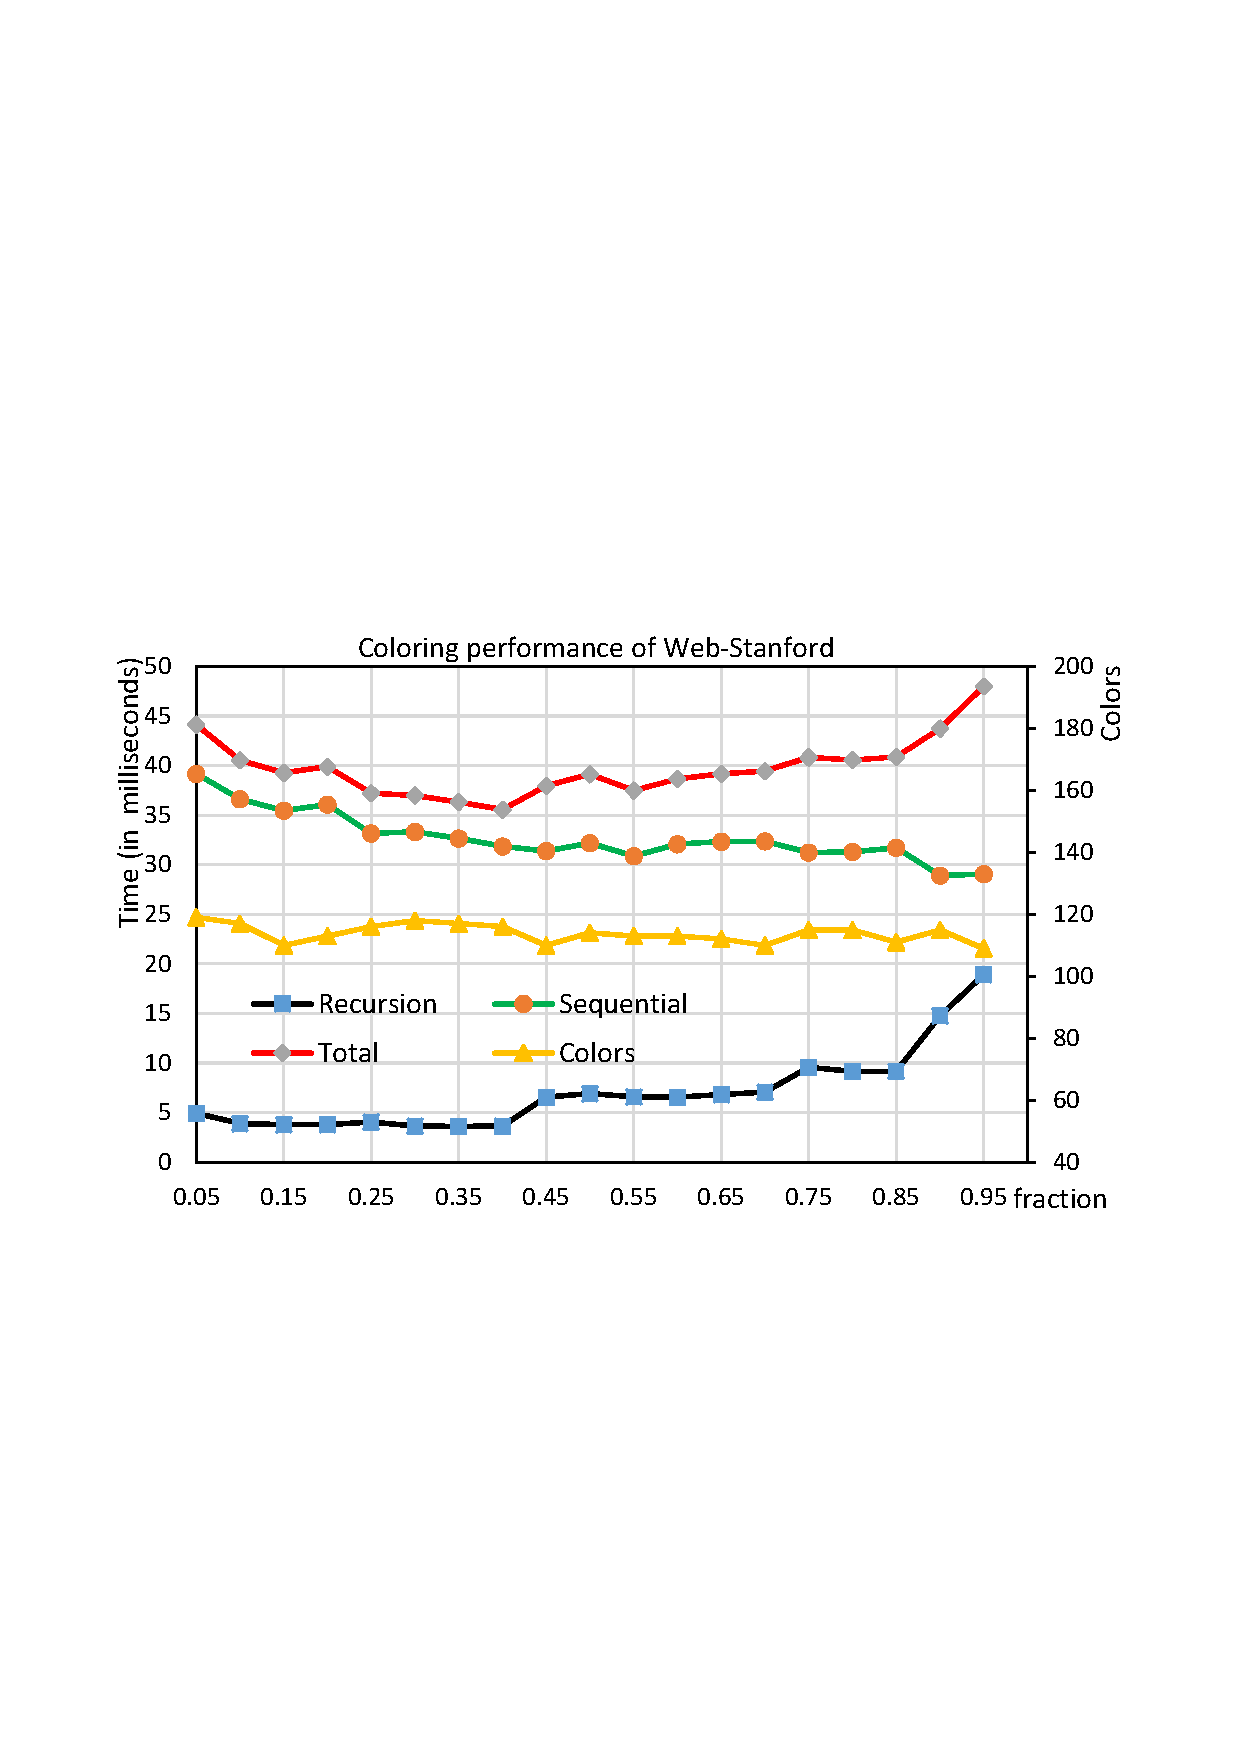
\includegraphics[scale=0.2]{figure/exp/web-s.pdf}
	}
	\subfloat[DBLP]{
		\label{fig:dblp}
		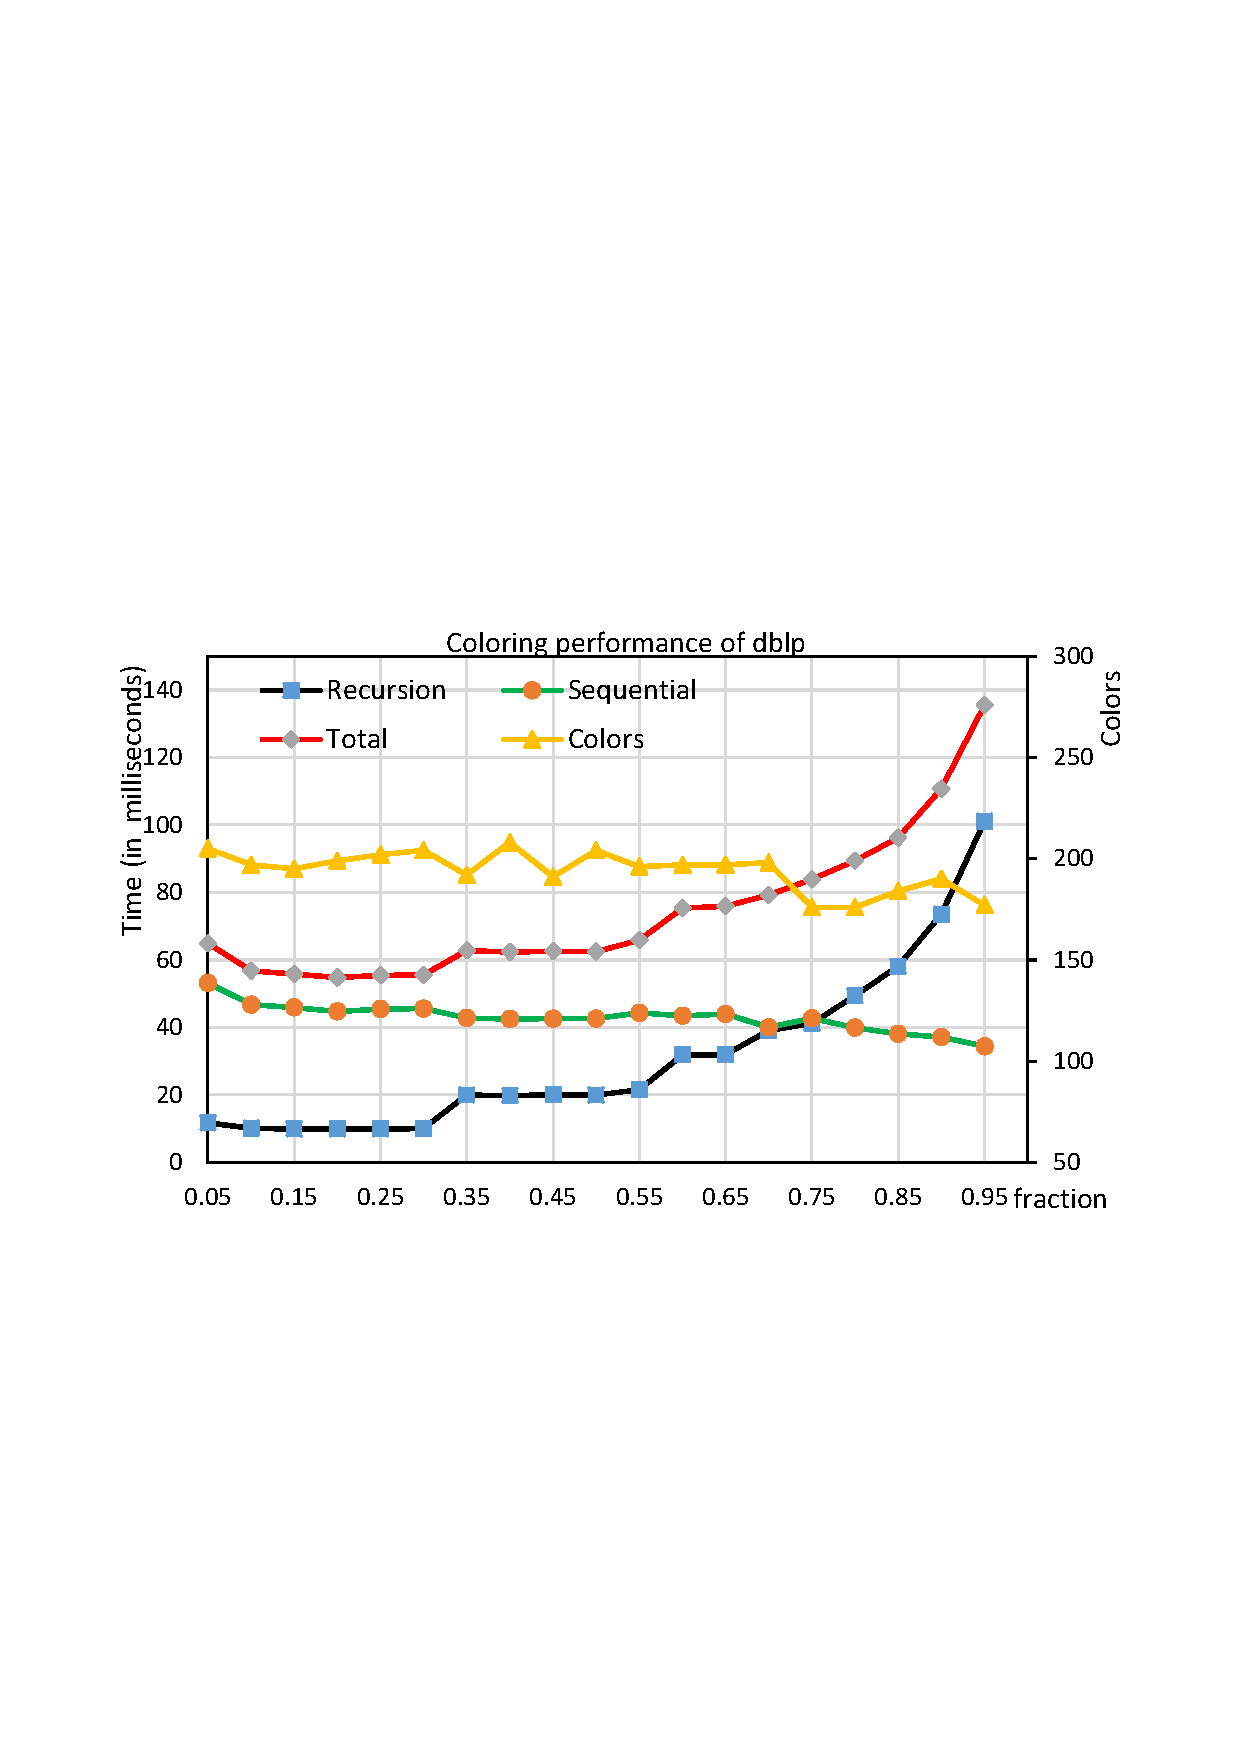
\includegraphics[scale=0.2]{figure/exp/dblp.pdf}
	} 
	\subfloat[Youtube]{
		\label{fig:youtube}
		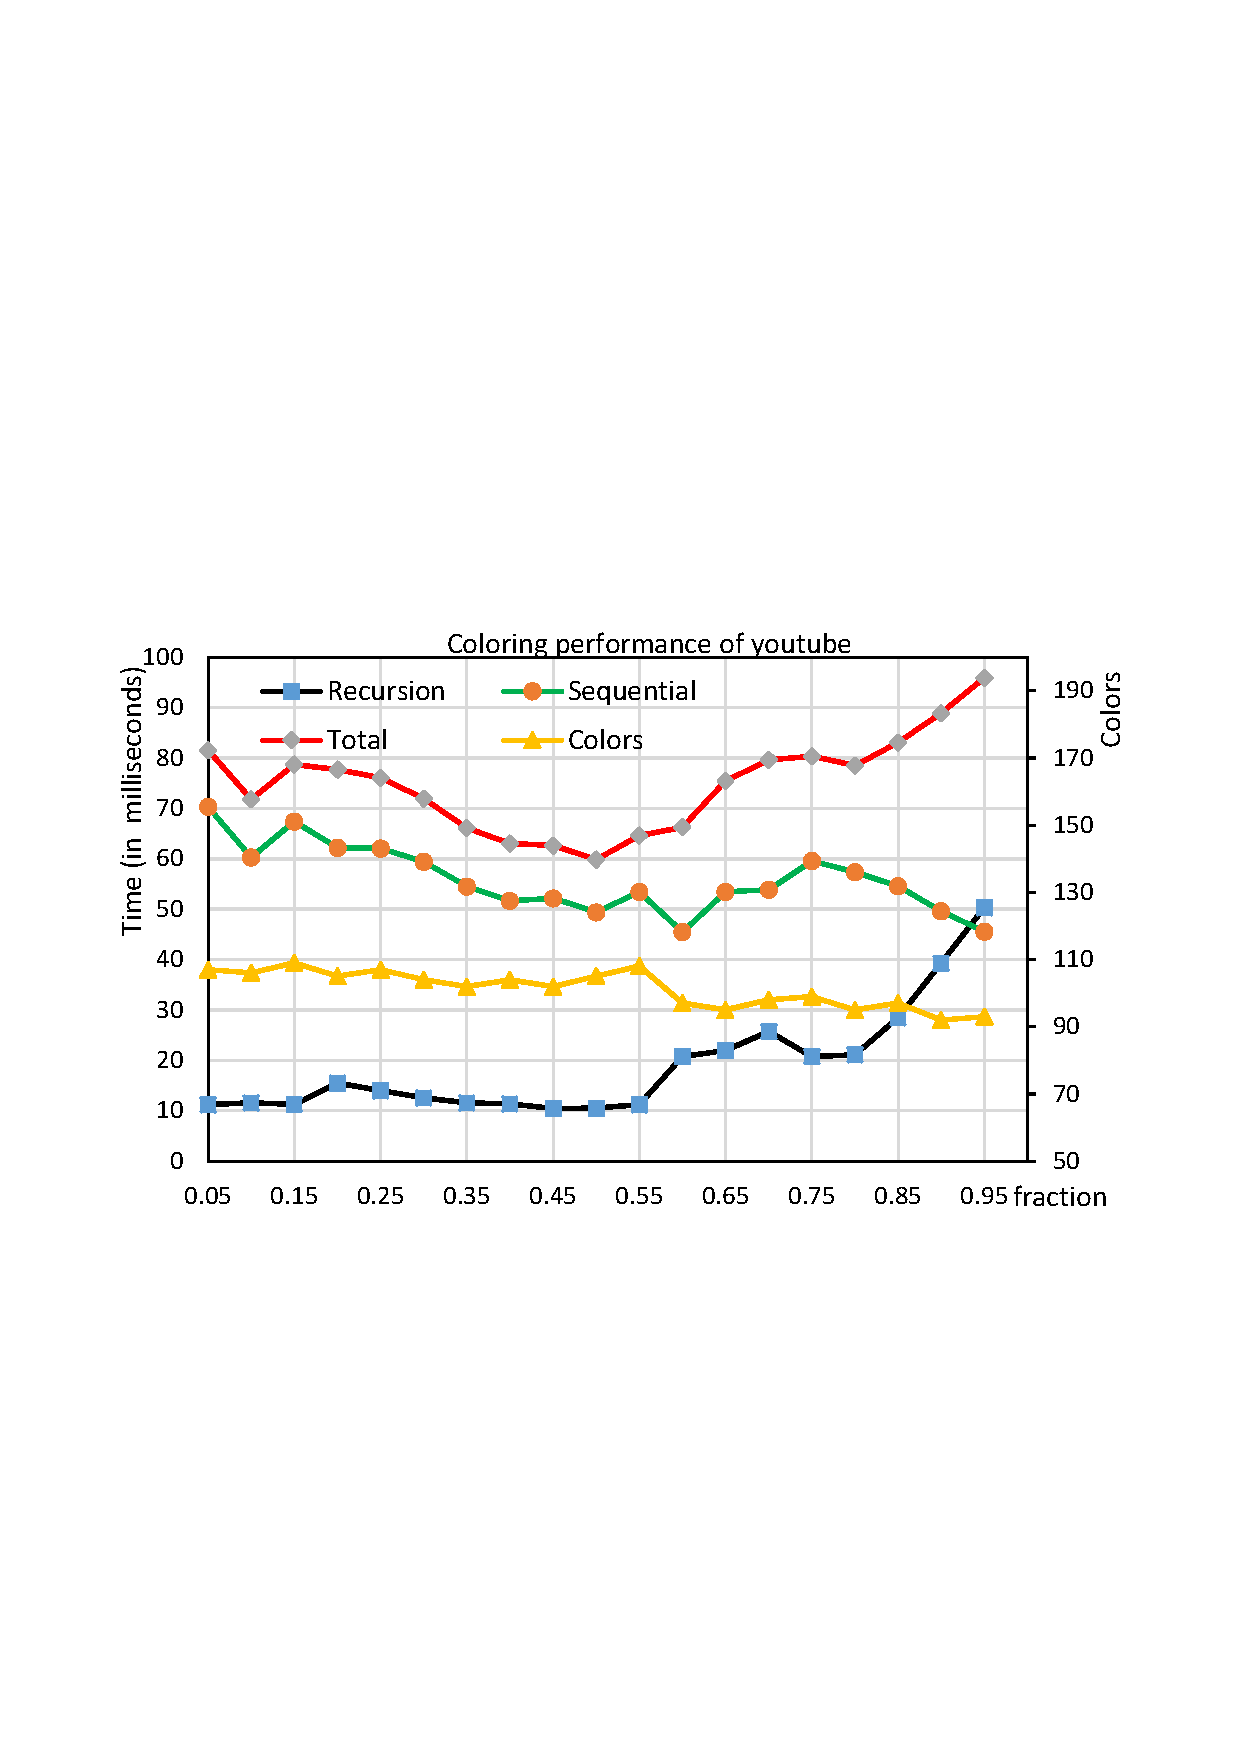
\includegraphics[scale=0.2]{figure/exp/youtube.pdf}
	}
	\subfloat[RoadNet]{
		\label{fig:roadnet}
		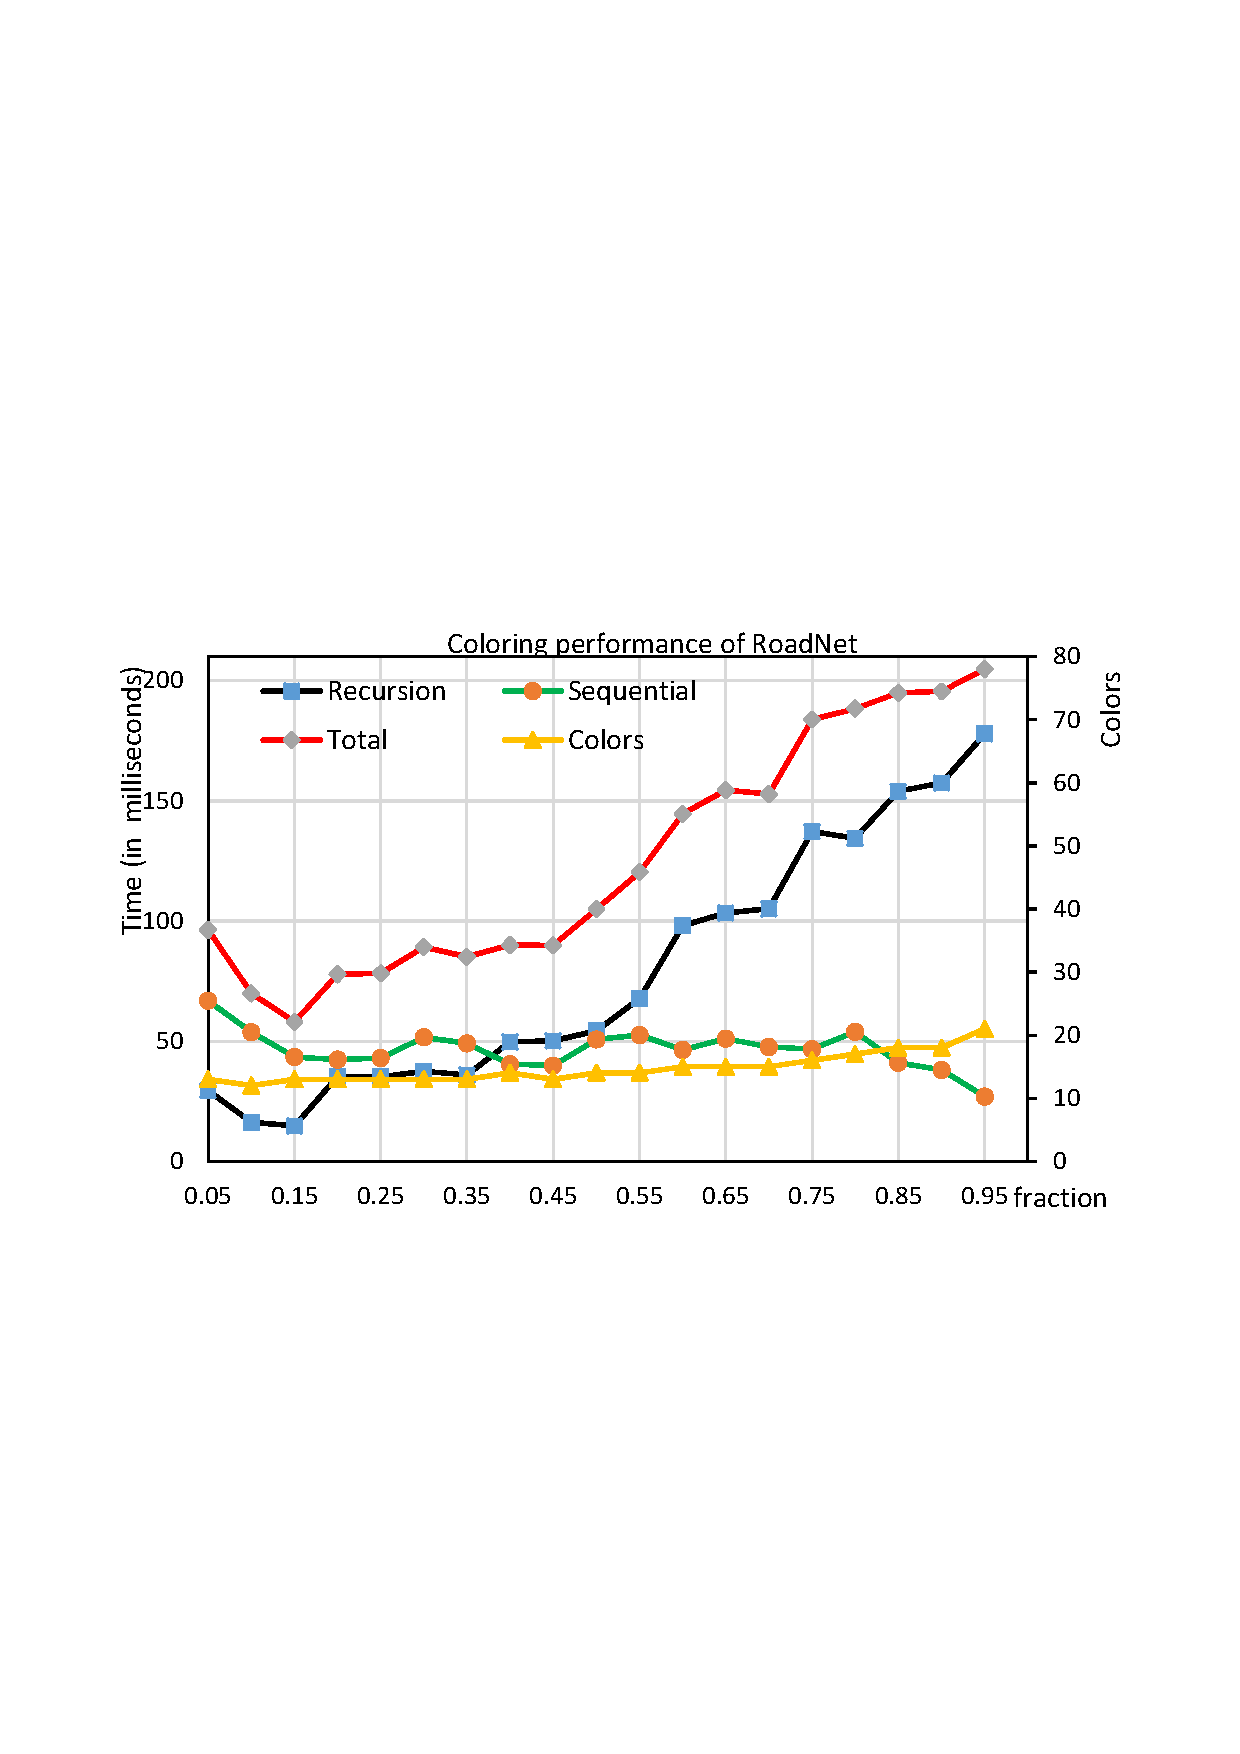
\includegraphics[scale=0.2]{figure/exp/roadnet.pdf}
	}
	\subfloat[Wiki]{
		\label{fig:wiki}
		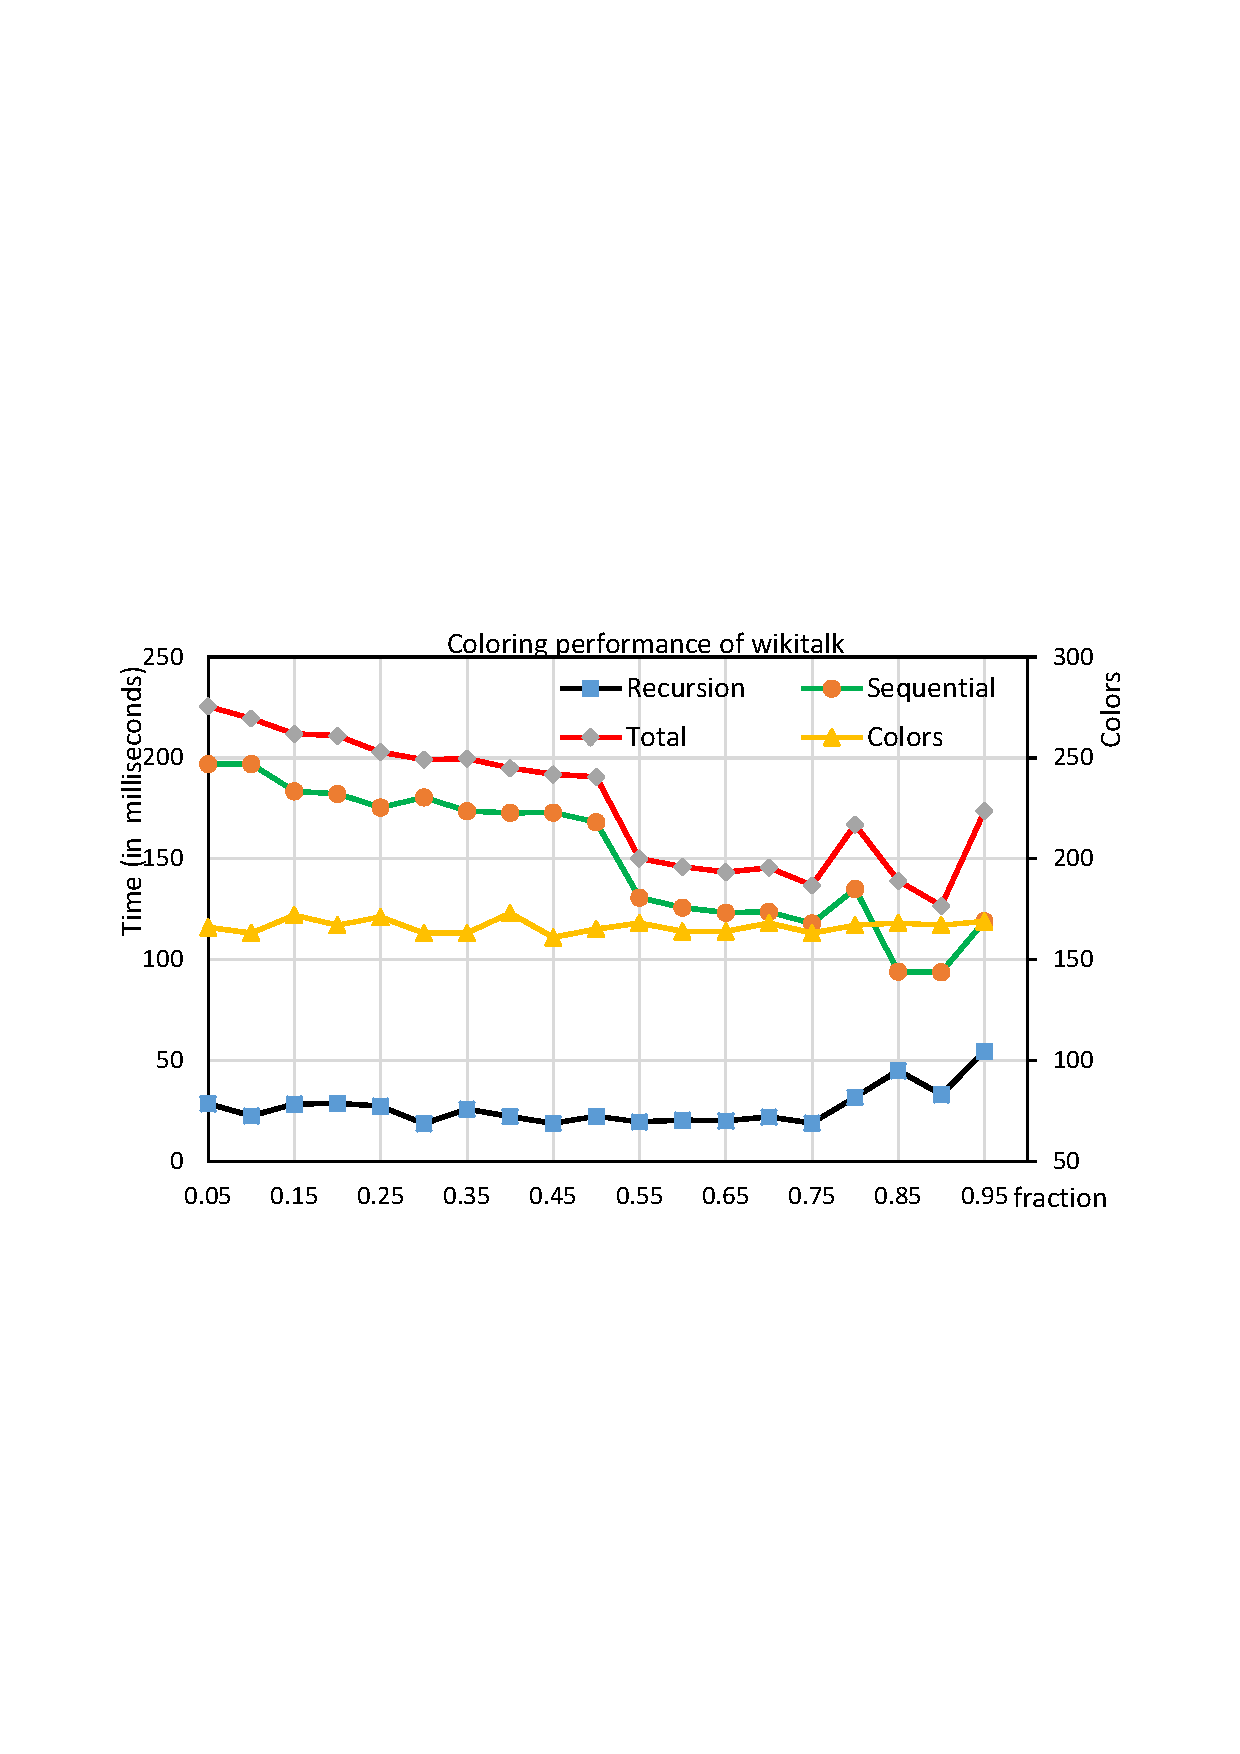
\includegraphics[scale=0.2]{figure/exp/wiki.pdf}
	}\\
	\subfloat[LiveJournal]{
		\label{fig:livejournal}
		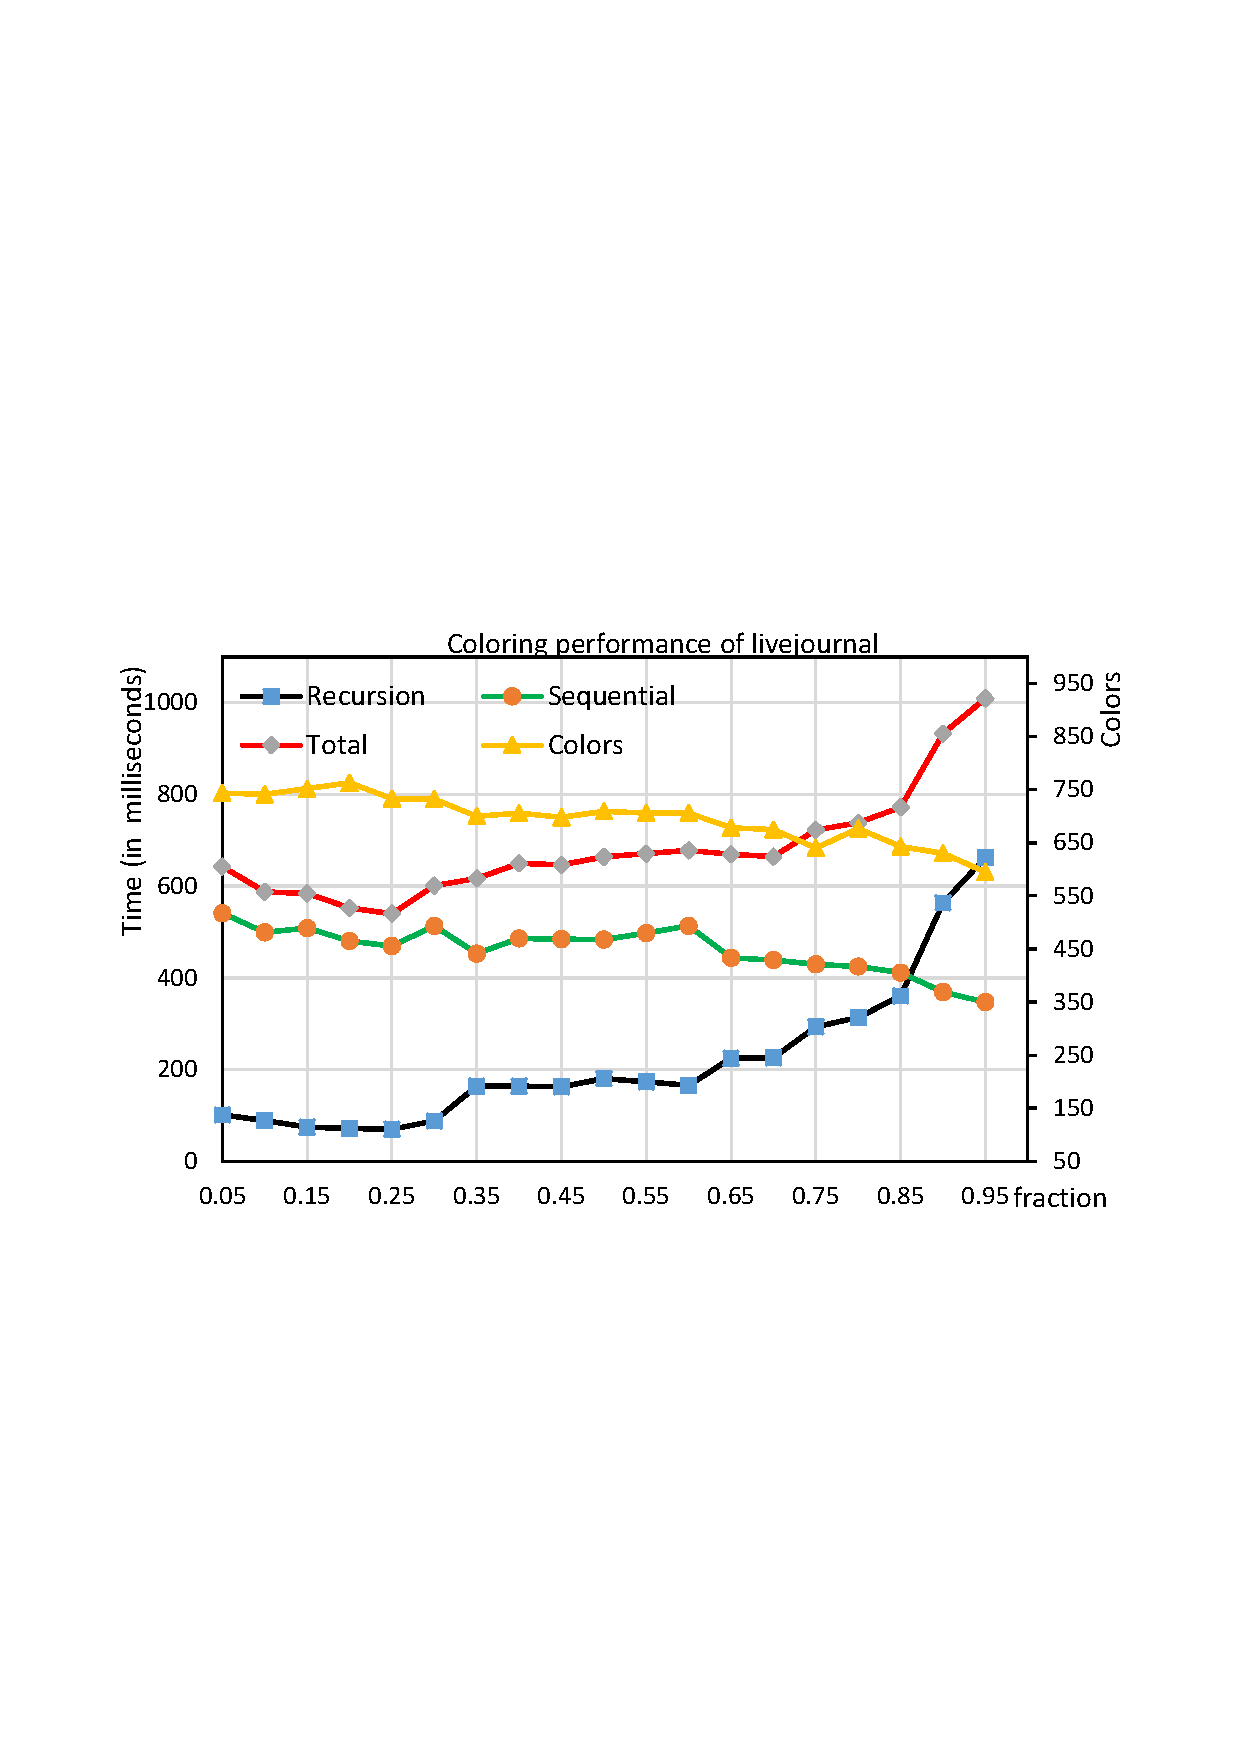
\includegraphics[scale=0.2]{figure/exp/livejournal.pdf}
	}
	\subfloat[RMAT]{
		\label{fig:rmat}
		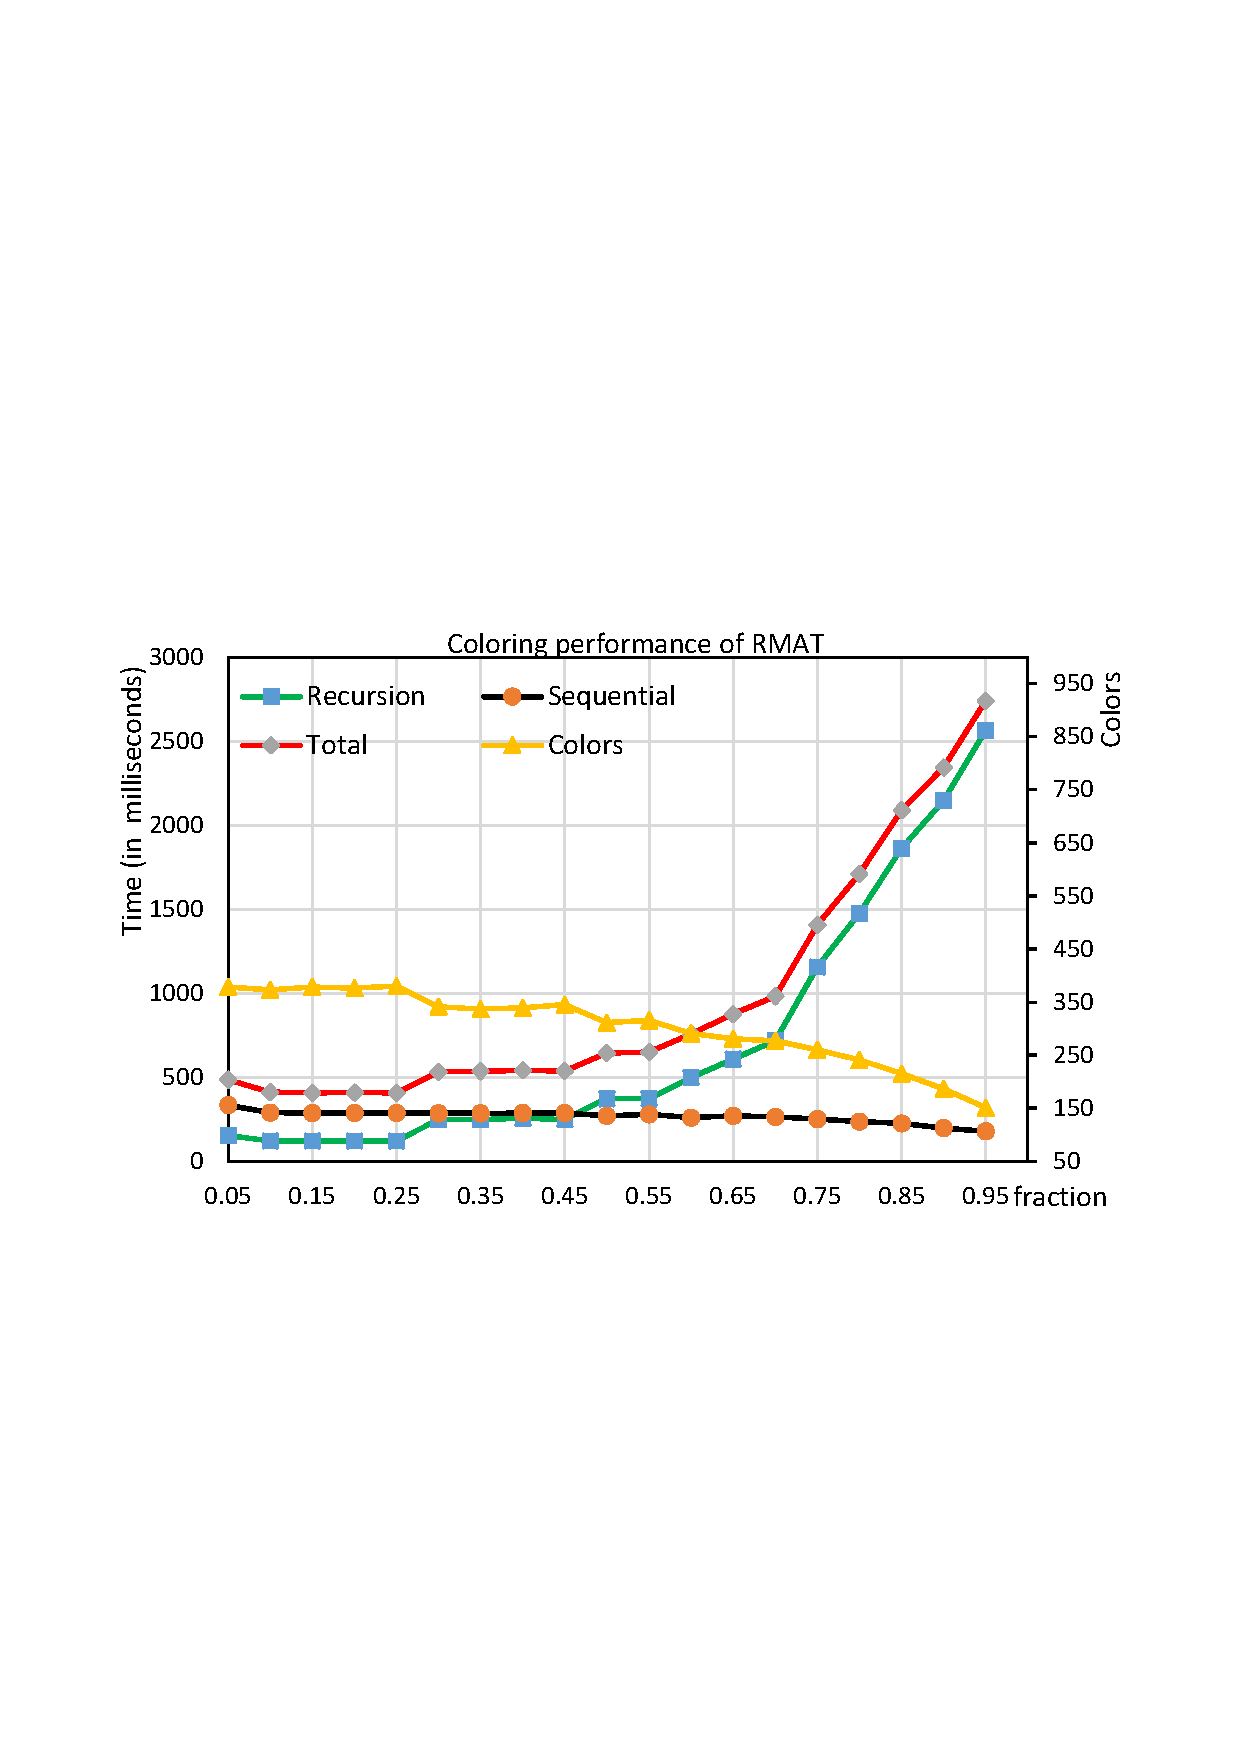
\includegraphics[scale=0.2]{figure/exp/rmat.pdf}
	}%
	\subfloat[RandomGraph]{
		\label{fig:random}
		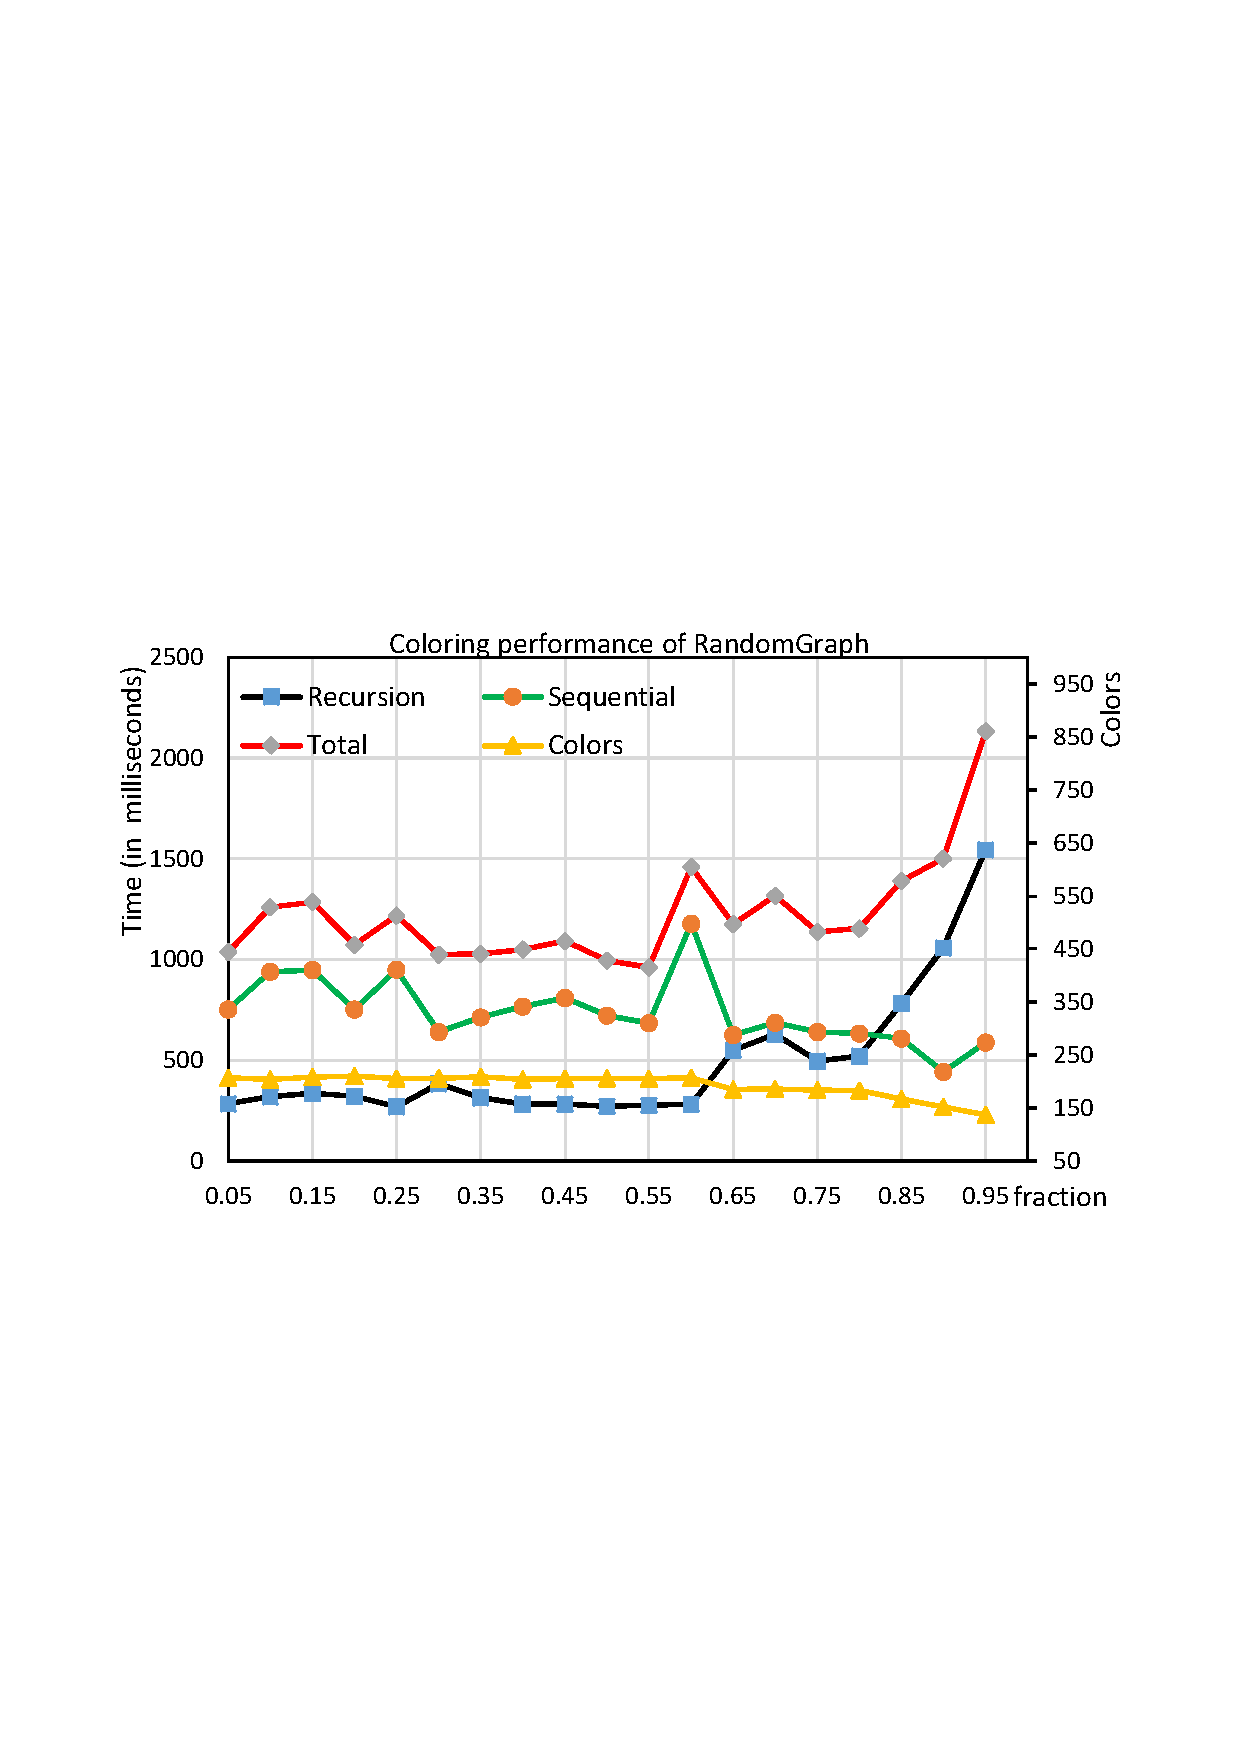
\includegraphics[scale=0.2]{figure/exp/random.pdf}
	}
	\subfloat[Twitter]{
		\label{fig:twitter}
		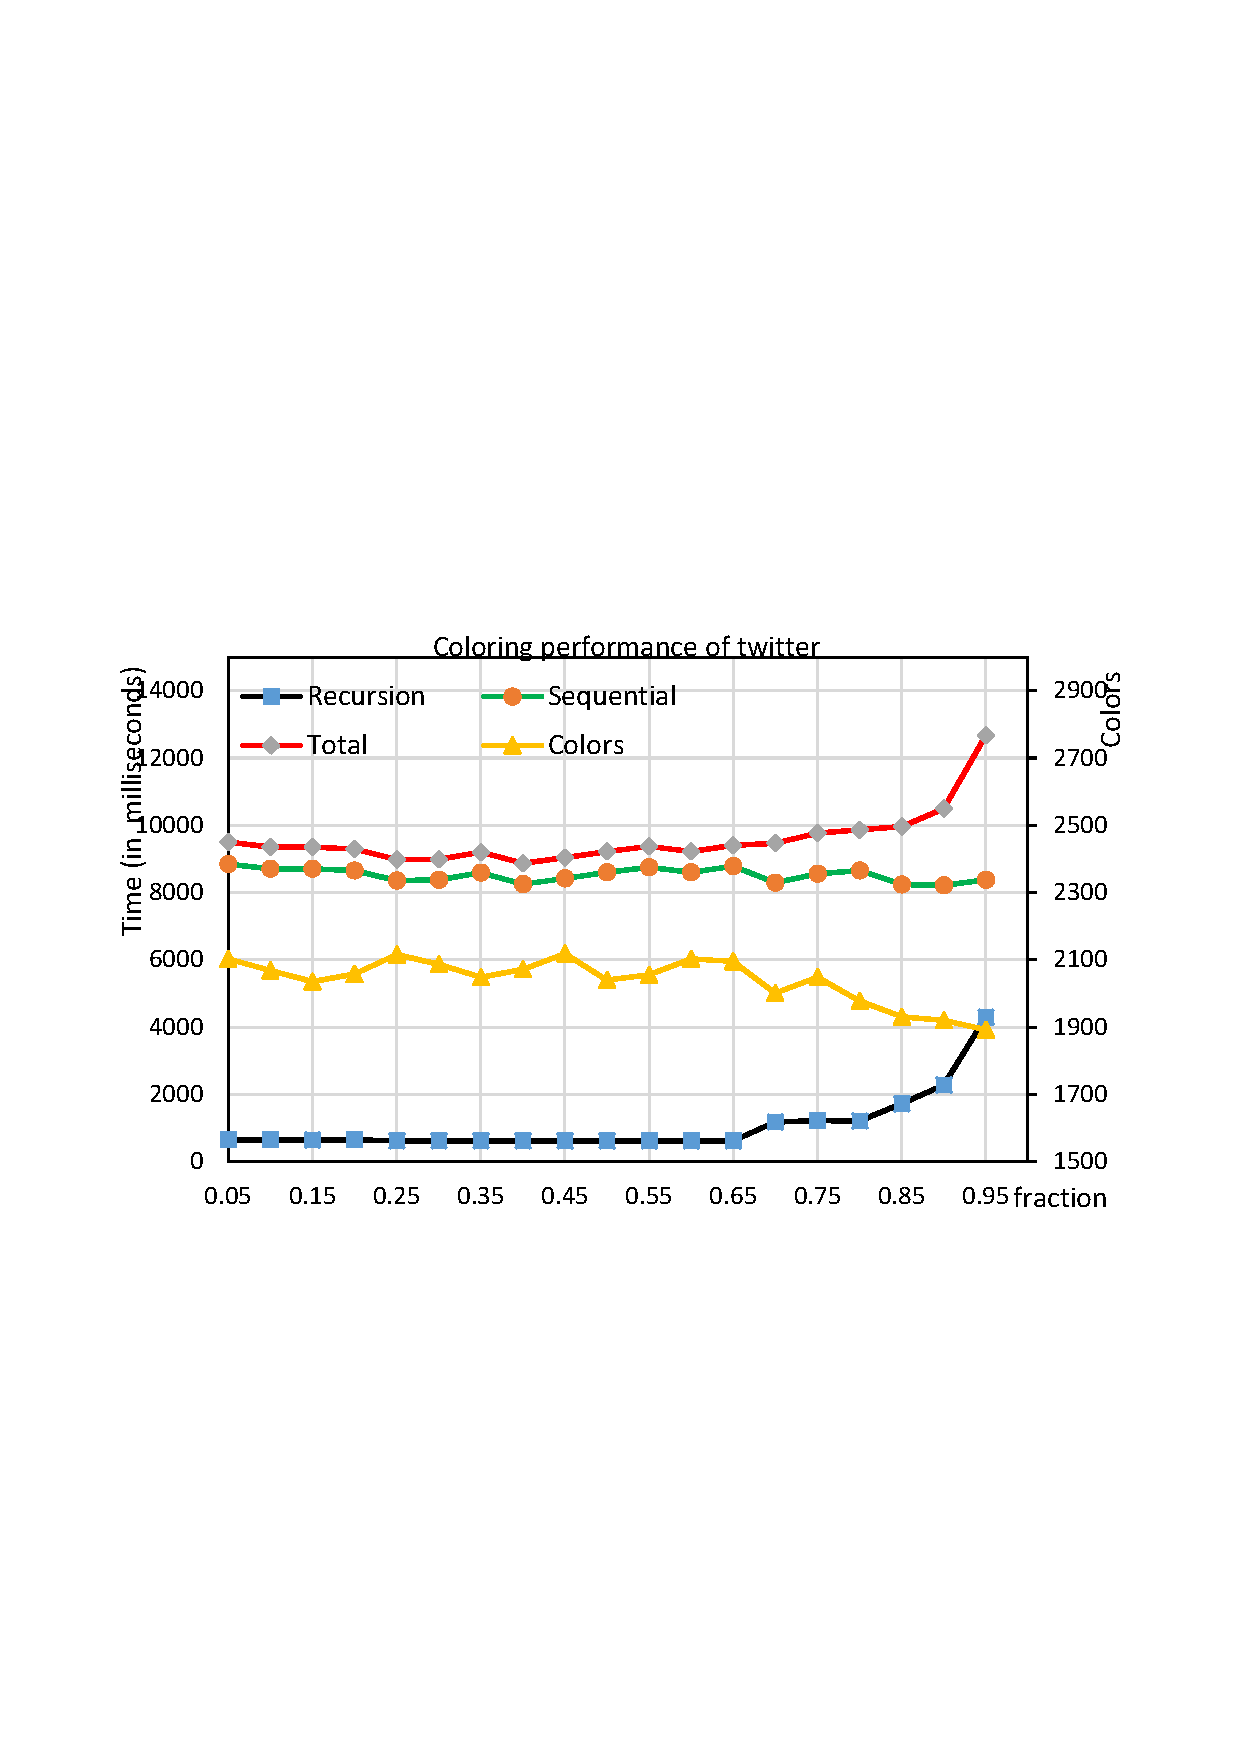
\includegraphics[scale=0.2]{figure/exp/twitter.pdf}
	}%
	\subfloat[Webbase]{
		\label{fig:webbase}
		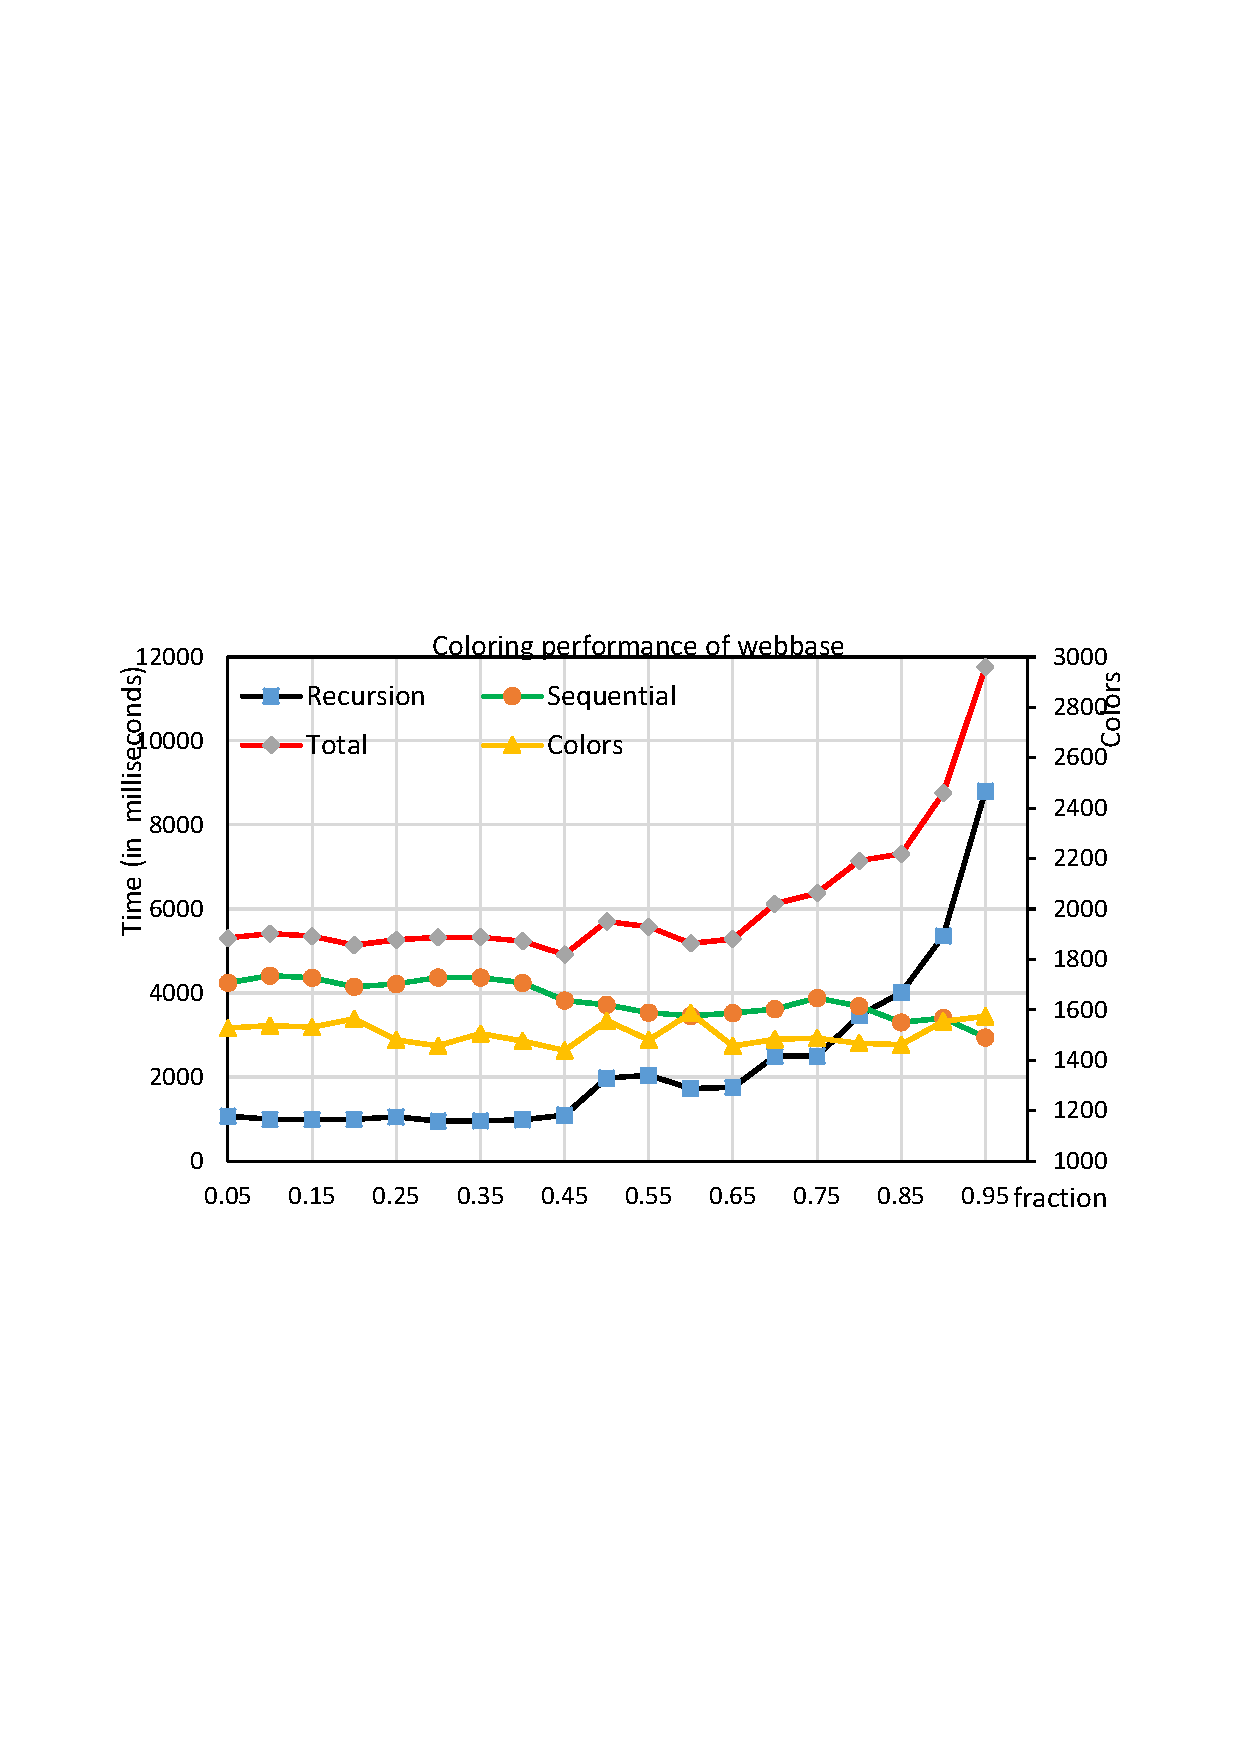
\includegraphics[scale=0.2]{figure/exp/webbase.pdf}
	}
	\caption{Coloring time with different \emph{fraction}. 
		X-axis is the value of \emph{fraction} and the Y-axis is the coloring time in milliseconds. Sequential Part means the time spent by the sequential spread stage of the coloring algorithm while the recursion part means the time by the recursion stage. The parameter \emph{fraction} indicates the ratio of the number of colored vertices in the recursion stage to the number of total vertices in the graph.}
	\label{fig:coloring}
\end{figure*}

In order to find a suitable value of the parameter $fraction$, which is used to control when the execution of Feluca is switched from the recursion stage to the sequential spread stage, we designed a set of experiments for different datasets with different value of fractions. The execution time of these two stages in Feluca with different \emph{fraction} values are shown in figure \ref{fig:coloring}. The left side y-axis in figure \ref{fig:coloring} is the coloring time in milliseconds, while the y-axis at the right side is the number of colors. The red line with gray diamond dots shows the total coloring time of Feluca, while the black line and the green line show the coloring times of the recursion and the sequential spread stage, respectively. The number of colors is shown by the yellow line with triangle dots.

We can make the following observations from figure \ref{fig:coloring}.
\begin{enumerate}
	\item The sequential spread stage is most time consuming with a small $fraction$ value, which means there are very few vertices colored in the recursion stage. According to the definition in section \ref{two-stage}, $\lambda = \frac{\sum_{j=1}^i{N_j}}{N}$ is the coloring rate in the recursion stage. When $\lambda \leq fraction =0.5$, it means there are a half vertices colored in the recursion stage while the other half are colored in the sequential spread stage. Figure \ref{fig:coloring} shows that the execution time of the recursion stage is much smaller than that of the sequential spread stage with all the power-law graphs, which means the recursion algorithm is much faster than the sequential spread algorithm. On the contrary, the recursion method needs more time with a big $fraction$ value, which means there are more conflicts occurred at the end of the  recursion stage.
	\item Feluca can achieve good performance on both power-law graphs and random graphs with a small number of colors.	
	\item Figure \ref{fig:coloring} shows that the execution time of Feluca is a convex function over $fraction$. Hence, Feluca can achieve the best coloring time when the derivative of the execution time function is close to 0. The derivative of the execution time function can be approximated as $\Delta t = \frac{t_i - t_{i-1}}{fraction_i - fraction_{i-1}}$. It can be assumed that the execution times of two consecutive iterations are the almost same. Then, Feluca switches from the recursion stage to the sequential spread stage when the number of active vertices is the same as the number of conflicting vertices in two consecutive iterations. 
\end{enumerate}

The recursion method becomes less efficient in in the later iterations, which is known as the long tail problem. Since Feluca assigns the colors to the conflicting vertices following the edges directions, most conflicting vertices can find suitable colors in the first few iterations. However, after a majority of vertices find the suitable colors, these colored vertices will have impact on the colors of the remaining vertices. This causes a small number of remaining vertices to change their colors repeatedly in later iterations and therefore shows down the progress. This is why Feluca switches from the recursion stage to the sequential spread stage when the condition stated in the last observation made from figure \ref{fig:coloring} is met.

\subsection{Comparison Against the State-of-the-art Techniques}

\begin{table*}[hpt]
\centering
\caption{Execution time for different coloring algorithms (in milliseconds)}
\label{tab:algs}
\begin{threeparttable}
\resizebox{\linewidth}{!}{
\begin{tabular}{|l|r|r|r|r|r|r|r|r|r|r|r|r|r|r|}
\hline
\multirow{2}{*}{Datasets} &\multicolumn{2}{c|}{CPU\_Greedy}	&\multicolumn{2}{c|}{Feluca}	&\multicolumn{2}{c|}{JPL}	&\multicolumn{2}{c|}{kokkos\_MIC}	&\multicolumn{2}{c|}{kokkos}	&\multicolumn{3}{c|}{cuSPARSE}\\ \cline{2-14} % &\multicolumn{1}{c|}{\multirow{2}{*}{Speedup}} \\ 
                  &\multicolumn{1}{c|}{Time} &\multicolumn{1}{c|}{Color}	&\multicolumn{1}{c|}{Time} &\multicolumn{1}{c|}{Color}	&\multicolumn{1}{c|}{Time} &\multicolumn{1}{c|}{Color} 	&\multicolumn{1}{c|}{Time} &\multicolumn{1}{c|}{Color}	&\multicolumn{1}{c|}{Time} &\multicolumn{1}{c|}{Color} 	&\multicolumn{1}{c|}{Time} &\multicolumn{1}{c|}{Color} &\multicolumn{1}{c|}{\tabincell{l}{Incorrect \\ Vertices}}\\ \hline%		&\multicolumn{1}{c|}{}\\ \hline
 web-Stanford			&103.955					&149					&\textbf{28.810}		&92					&1121.790		&169	&2200.720		&\textbf{45}&50.765			&\textbf{45}	&1463.250					&95						&134993\\
 dblp							&322.065					&119					&\textbf{42.388}		&139				&787.762		&121	&6106.440		&119				&183.034		&119					&541.429					&\textbf{70}	&933161\\
 youtube					&216.808					&\textbf{43}	&\textbf{58.777}		&57					&1409.490		&262	&3022.930		&46					&230.806		&45						&617.205					&103					&283515\\
 RoadNet					&145.619					&\textbf{5}		&\textbf{12.524}		&6					&806.787		&13		&4893.600		&5					&162.546		&6						&531.205					&32						&1953477\\
 Wiki-Talk				&774.658					&97						&\textbf{122.464}		&95					&8703.570		&489	&5042.670		&67					&631.069		&\textbf{65}	&818.762					&159					&184167\\
 soc-LiveJournal	&4805.730					&328					&\textbf{448.574}		&551				&11000.500	&646	&63284.500	&251				&1629.902		&251					&1792.390					&\textbf{184}	&2437231\\
 RMAT16\_2				&8965.460					&75						&\textbf{485.550}		&410				&18774.900	&316	&163517			&26					&4454.264		&\textbf{23}	&6910.610					&129					&6966819\\
 random-graph			&9076.560					&94						&\textbf{353.643}		&86					&17264.300	&334	&96557.300	&25					&2968.788		&\textbf{22}	&9264.060					&112					&4804572\\
 twitter-2010			&83796.800				&918					&\textbf{5040.660}	&947				&null				&null	&728099			&\textbf{679}&null			&null					&41201.3					&917	&22396212\\
 webbase-2001			&343404						&1507					&\textbf{2729.500}	&1559				&null				&null	&940540			&1226				&null			&null						&264022						&\textbf{412}	&104173619\\\hline
 Feluca Speedup		&\multicolumn{2}{c|}{3.61$\times$ -- 125.81$\times$}	&\multicolumn{2}{c|}{--}			&\multicolumn{2}{c|}{18.58$\times$ -- 71.07$\times$}		&\multicolumn{2}{c|}{41.18$\times$ -- 344.58$\times$} &\multicolumn{2}{c|}{1.76$\times$ -- 12.98$\times$}	&\multicolumn{3}{c|}{4$\times$ -- 96.73$\times$}\\\hline
\end{tabular}}
\begin{tablenotes}
\item {Note: }{Null means that the system cannot process such a dataset. CPU\_Greedy and kokkos\_MIC are run on the Intel(R) Xeon(R) \\ 
E5-2670 CPU with 16 threads, while others are run on \texttt{NVIDIA Tesla K20m GPU}. Reference \cite{Manycore} shows that kokkos can achieve the \\ 
best performance by using the edge-based coloring method. So we set the parameter \texttt{--algorithm} as \texttt{COLORING\_EB} for kokkos\_MIC \\
and kokkos in our experiments. 
%We also tried to run kokkos on \texttt{NVIDIA Tesla K20m GPU}, but failed. This may be due to the flaw in kokkos since the authors said ``sometimes the build system acts weird especially when configure options are changed''.
}
%\item {GPU. And the improvement is made based on Frog.}
\end{tablenotes}
\end{threeparttable}
\end{table*}

We compared Feluca with some recent researches, such as cuSPARSE, JPL ~\cite{nvidiaTR} and a CPU implementation of greedy coloring algorithm. Table \ref{tab:algs} shows the execution time and the number of colors used for all ten graphs. A performance value plotted in each graph is the average of 5 independent runs of the GPU-based solutions (Feluca, cuSparse, and JPL) or the average of 10 runs of the CPU based implementation.

The experimental results show that Feluca achieves up to 125.81$\times$ speed up over the CPU-based Greedy coloring algorithm, 111.98$\times$ speed up over the JPL algorithm and up to 96.73$\times$ speed up over the state-of-the-art cuSPARSE algorithm. For the reference, one of the recent researches \cite{Manycore} achieved only up to 1.5$\times$ speed up over cuSPARSE. 

Table \ref{tab:algs} shows that Feluca outperforms all other competitors in terms of run-time with all ten datasets. All these algorithms can generate a complete coloring plan except cuSPARSE, which is an incomplete coloring algorithm. For example, out of the 4,847,571 vertices in \texttt{soc-LiveJournal}, 41,652,230 vertices in \texttt{twitter-2010}, 118,142,155 vertices in \texttt{webbase-2001}, cuSPARSE assigns 2,437,231 and 22,396,212 and 104,173,619 vertices, respectively, to the same color. From another point of view, cuSPARSE does not choose another right color for the vertices when the conflicts occur. 41,652,230 vertices of \texttt{twitter-2010} are colored with 947 colors in Feluca while cuSPARSE only colored the 19,256,018 (46\% of all the vertices) vertices  using 917 colors and assigns the remaining 22,396,212 vertices to the same color. This is the main reason why cuSPARSE can achieve a fewer number of colors on \texttt{soc-LiveJournal, twitter-2010} and \texttt{webbase-2001}.

As described in section \ref{eliminate}, Feluca only focuses on the current vertex and their parents and does not search the entire color array to find the available color for the current vertex. Although this scheme avoids the use of atomic operations (hence improve the run-time performance), it may increase the number of used colors to some extent. Table \ref{tab:algs} shows cuSPARE can color the \texttt{soc-LiveJournal}, \texttt{twitter-2010} and \texttt{webbase-2001} datasets with the fewer colors than Feluca. The smaller color count by cuSPARSE is also due to incomplete nature of its solution. 

\subsection{The Color-centric Scheme in Feluca}
\label{perfo}

In this experiment, we implement Feluca with and without the color-centric paradigm. The experiment is designed to show the ratio of the number of conflicting vertices to the number of active vertices in each iteration. The experiment result is shown in figure \ref{fig:scale}. The figure shows that, without the color-centric paradigm the tested three datasets, \texttt{web-Stanford}, \texttt{youtube} and \texttt{RandomGraph}, need at least 24 iterations to converge. While with the color-centric paradigm, \texttt{RandomGraph} converged at the $7^{th}$ iteration and other two datasets converged at the $11^{th}$ iteration.

Figure \ref{fig:scale} also shows that with the color-centric paradigm, the ratio of the number of conflicting vertices to the number of active vertices in each iteration is no more than 45\% for \texttt{youtube} and \texttt{RandomGraph}, while the conflict ratio can increase to 80\% -- 87\% without the color-centric paradigm. The color-centric paradigm can avoid about 50\% conflicts for these two datasets. The conflict ratio of \texttt{web-Stanford} increased to 87\% at the $10^{th}$ iteration, while the conflict ratio is no more than 63\% with the color-centric paradigm.

\begin{figure}[h]
	\centering
		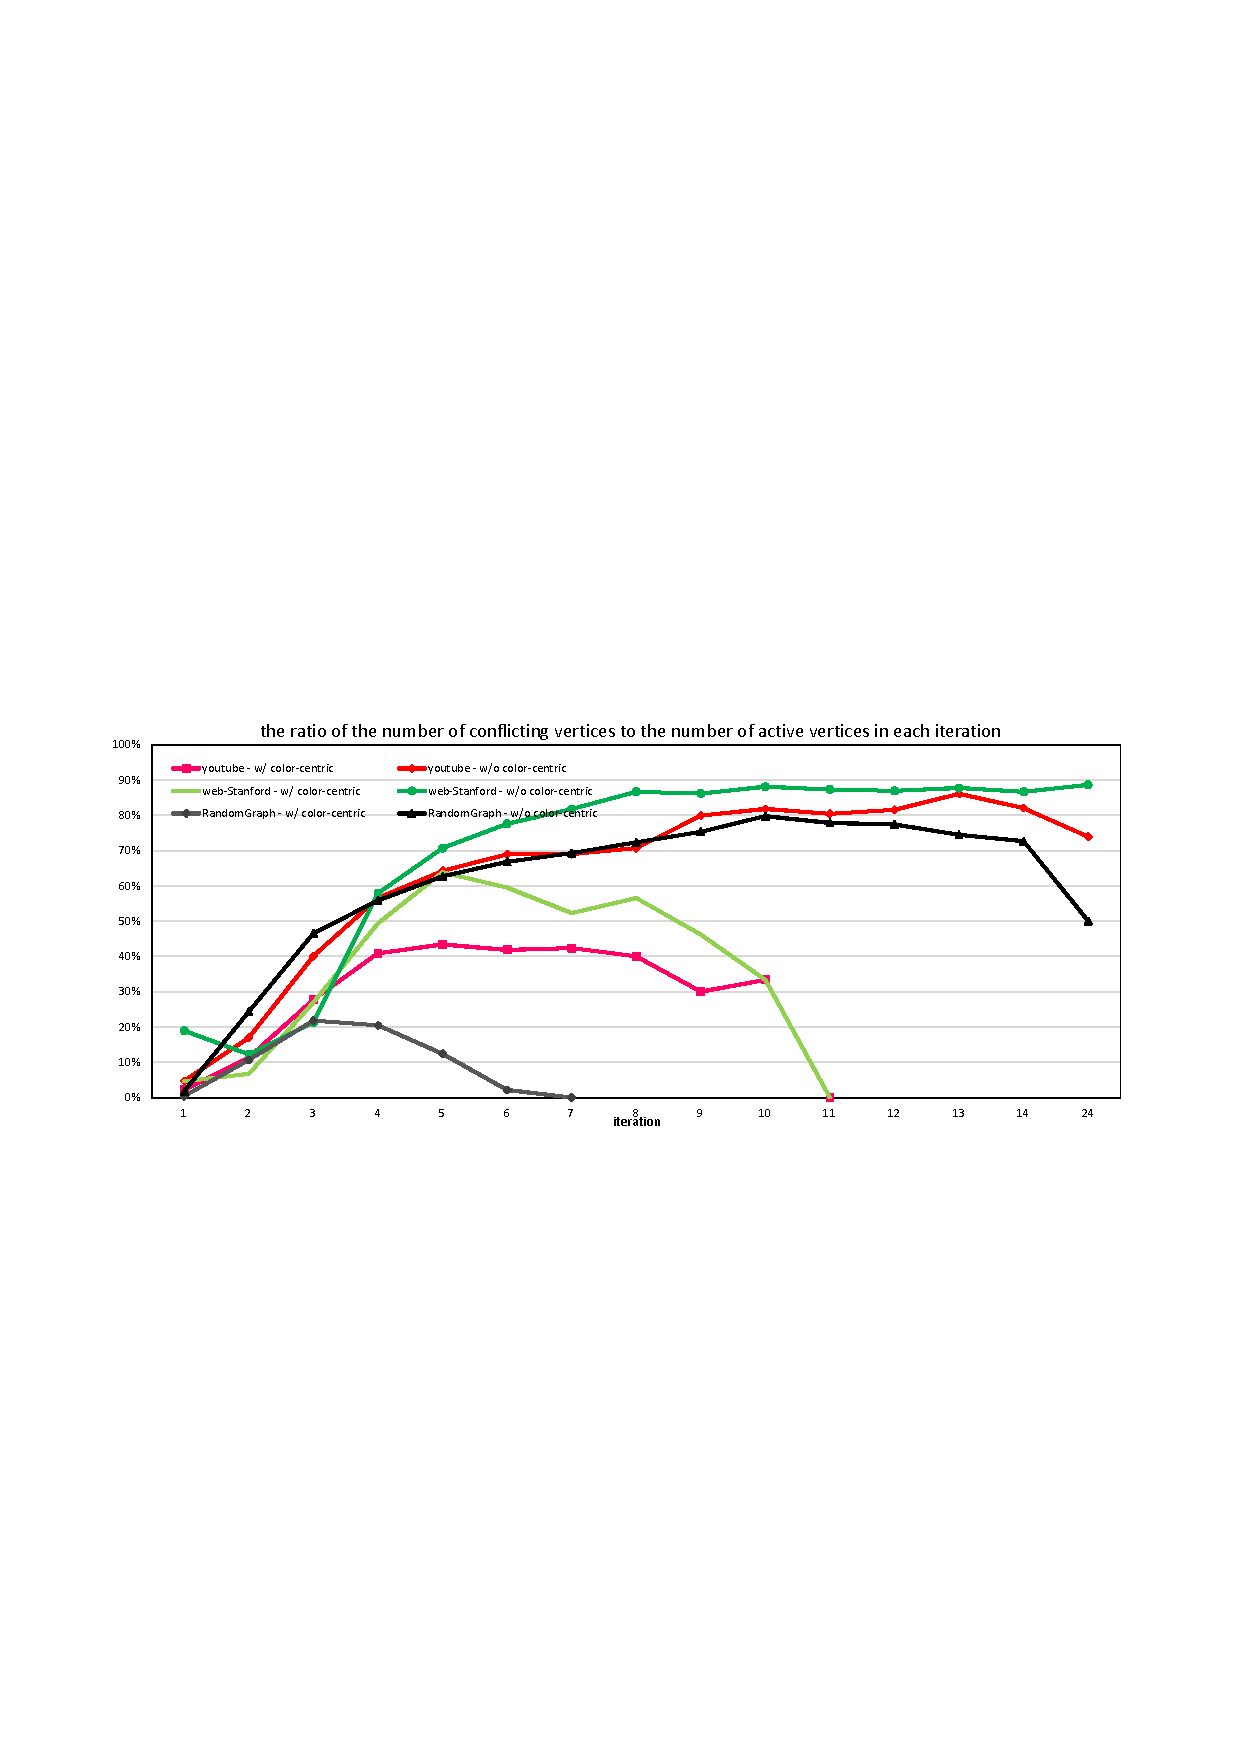
\includegraphics[scale=0.4]{figure/conflict_Feluca.pdf}
	\caption{The ratio of the number of conflicting vertices to the number of active vertices in each iteration with and without color-centric optimization}
	\label{fig:scale}%
\end{figure}

\begin{figure}[h]
	\centering
		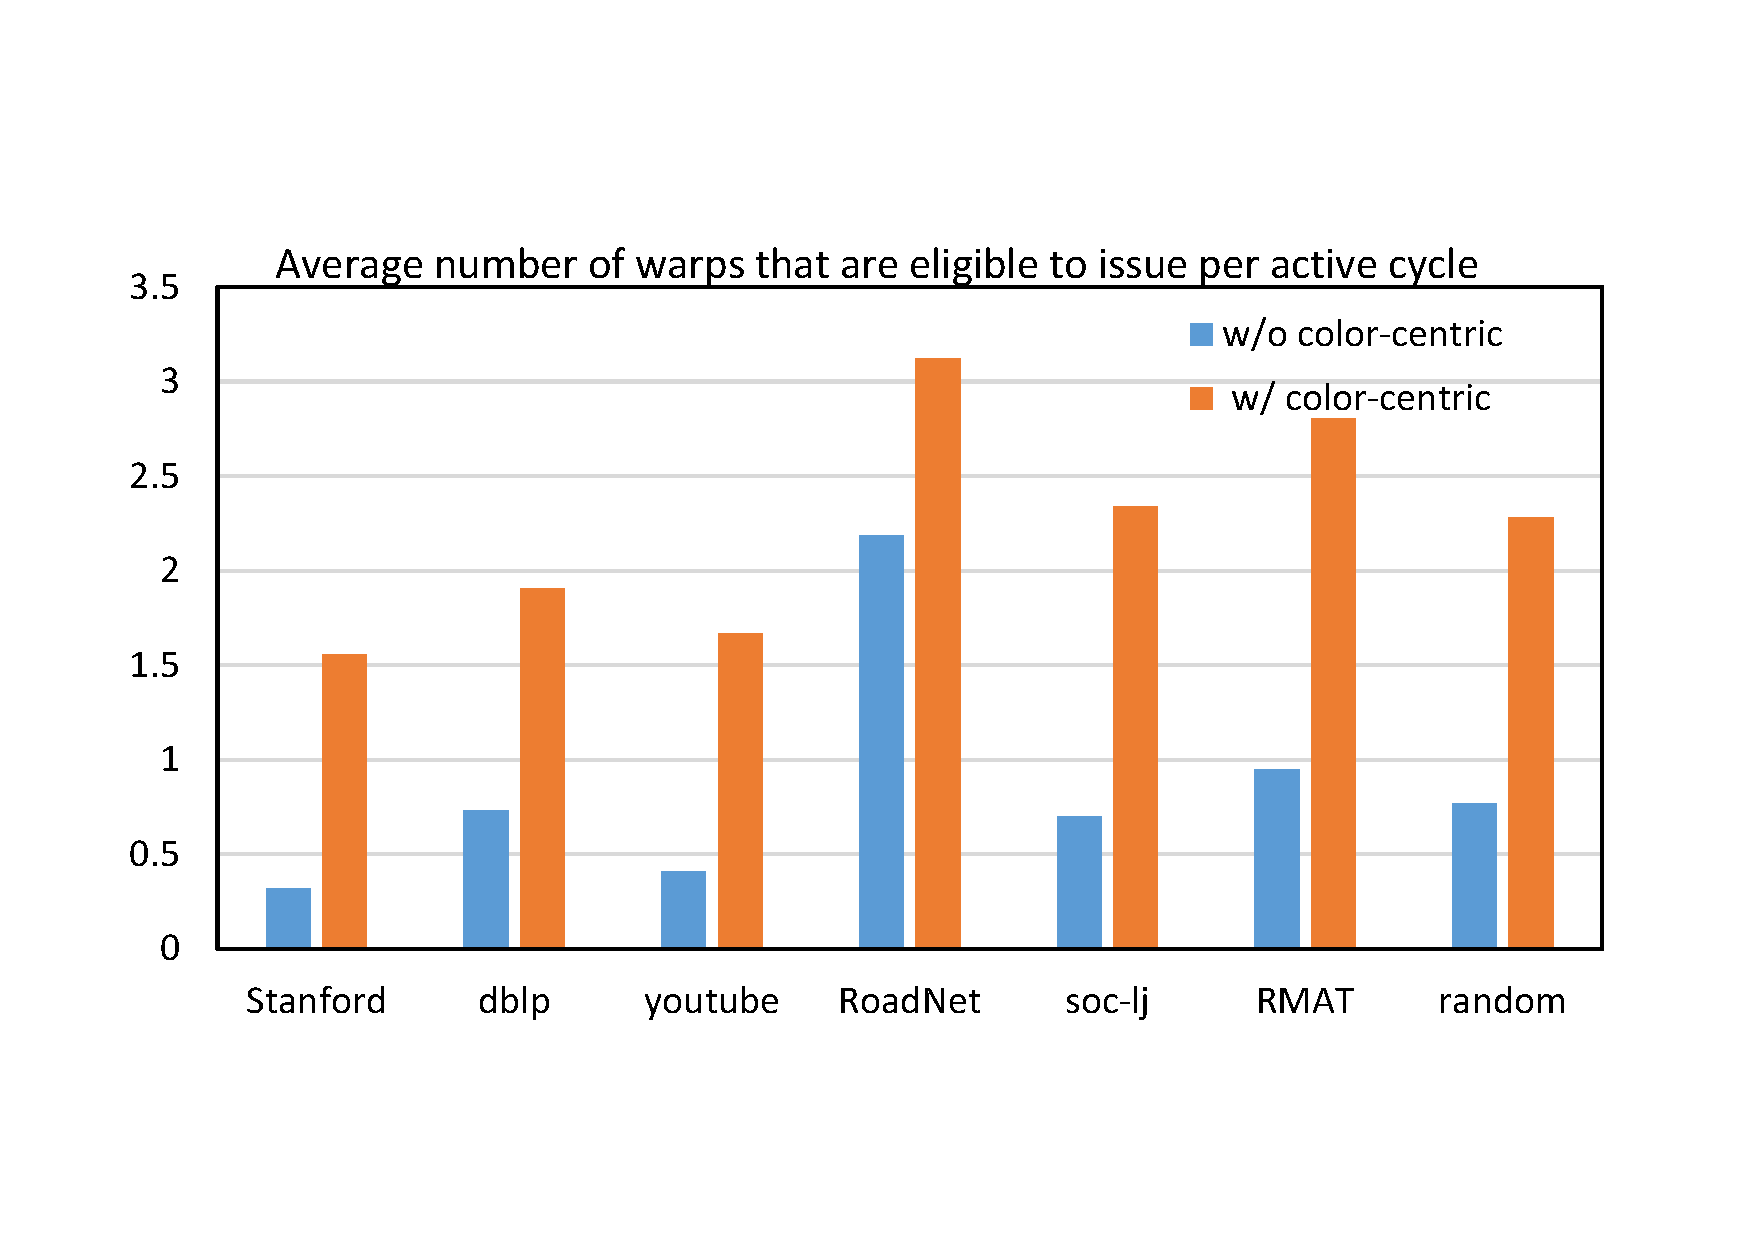
\includegraphics[scale=0.25]{figure/exp/warps.pdf}
	\caption{The average number of warps that are eligible to issue per active cycle with and without color-centric optimization}
	\label{fig:warps}%
\end{figure}

Figure \ref{fig:slot_utilization} shows the percentage of issue slots that issued at least one instruction, averaged across all cycles. The figure shows that the color-centric paradigm can improve the performance by 111\% (on RoadNet dataset) -- 410\% (on web-Stanford dataset), which indicates that more instruction were executed in every iteration by using the color-centric paradigm.

\begin{figure}[h]
	\centering
		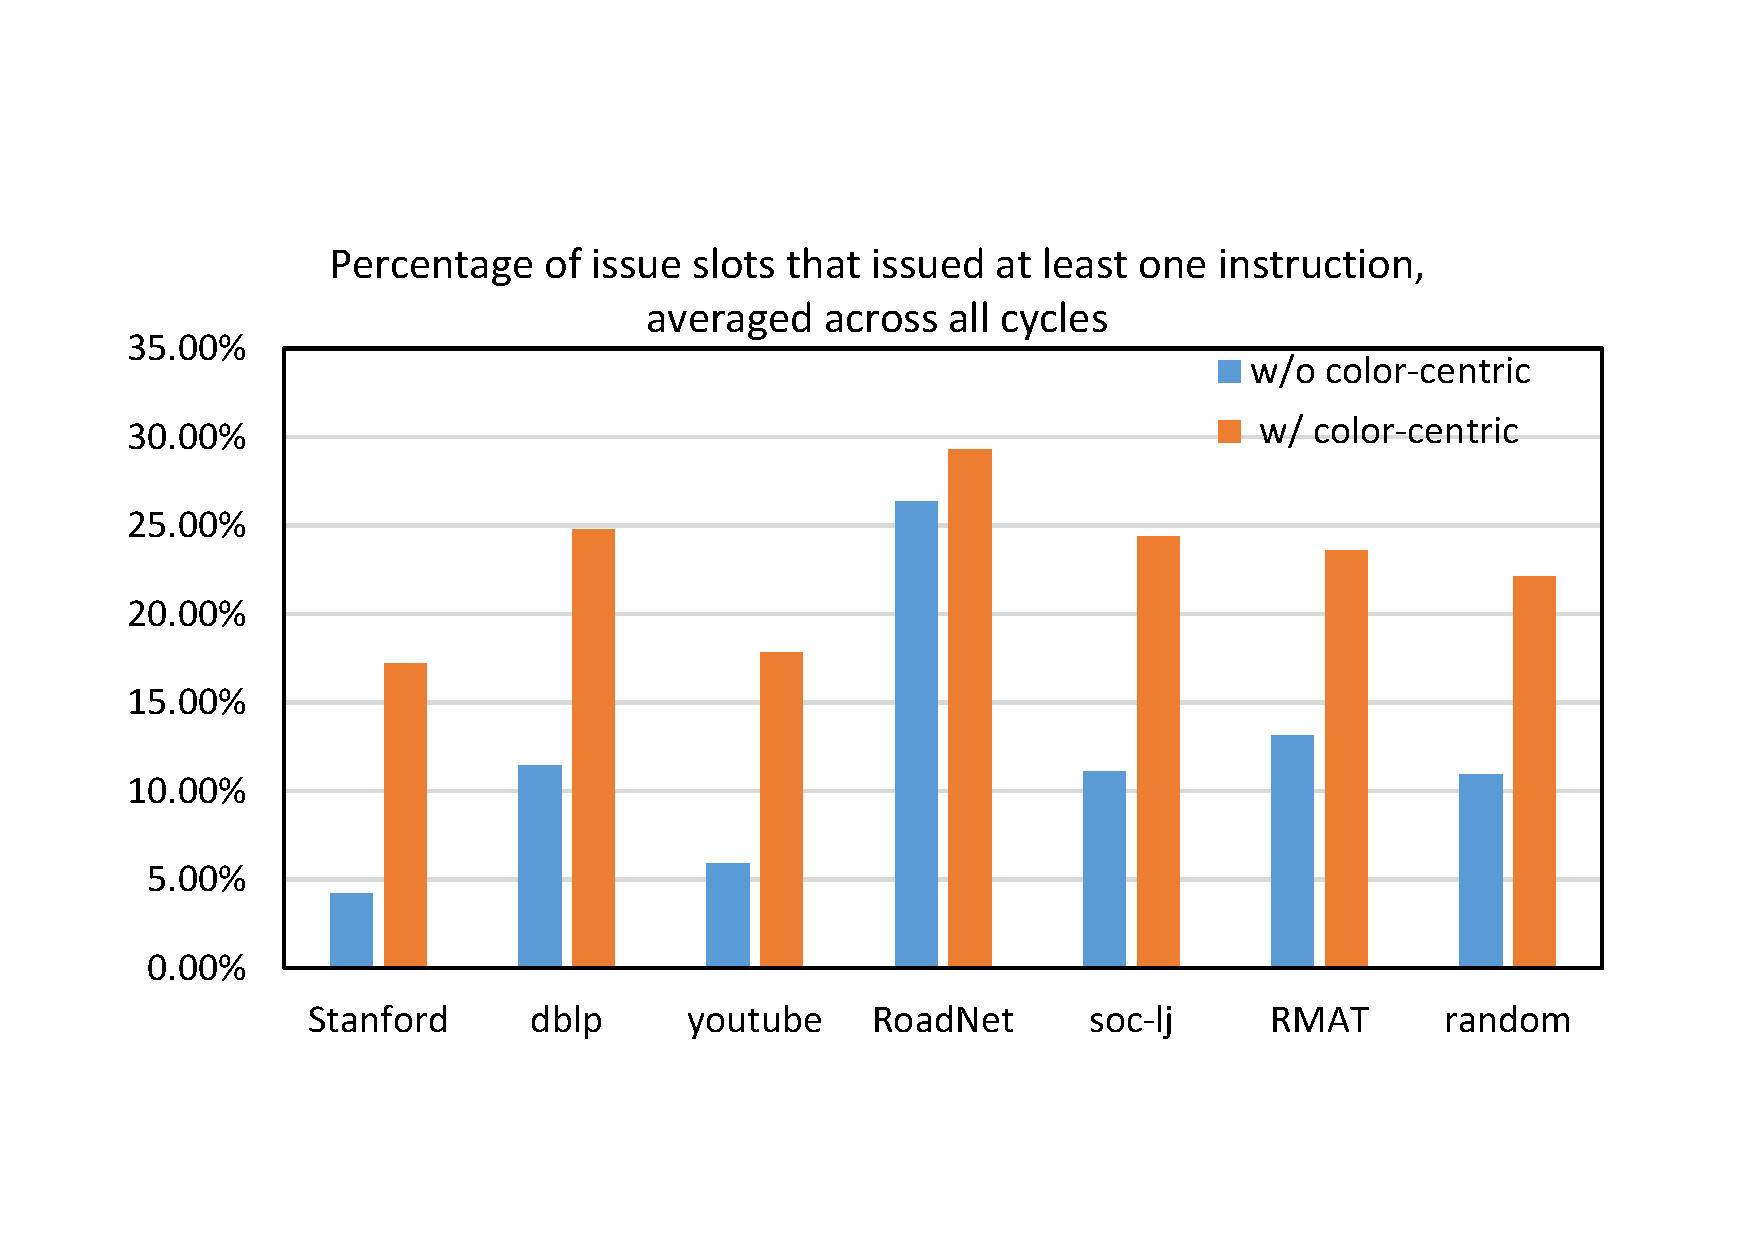
\includegraphics[scale=0.25]{figure/exp/slot_utilization.pdf}
	\caption{The percentage of issue slots that issued at least one instruction, averaged across all cycles, with and without the color-centric scheme}
	\label{fig:slot_utilization}%
\end{figure}

Figure \ref{fig:warps} plots the average number of warps that are eligible to issue per active cycle. Figure \ref{fig:slot_utilization} shows the percentage of the issue slots that issued at least one instruction  respectively. Figure \ref{fig:warps} shows that on the RoadNet dataset, the average number of warps in each active cycle is no more than 2.2 without the color-centric paradigm, while with the color-centric paradigm it increases to 3.12. On web-stanford dataset, the color-centric paradigm can improve the average number of warps in each active cycle by up to 4.9$\times$. These experiments show that the color-centric paradigm can improve the active warps in each execution cycle, which means the there are more active threads by using the color-centric paradigm.



\subsection{Running Feluca on Different GPU Devices}
\label{subsec.scalability}
In order to show the perforance of Feluca on three different GPU device, NVIDIA K20, NVIDIA K40 and NVIDIA P100. The configuration of NVIDIA K20 is the same as in pervious experiments.  There are 2880 CUDA cores and 12GB on-board memory in NVIDIA K40, and there are 3584 CUDA cores and 16GB on-board memory in NVIDIA P100. Figure \ref{fig:scale} shows the performance achieved by Feluca scales well with the  increase of the GPU capability.

\begin{figure}[h]
	\centering
		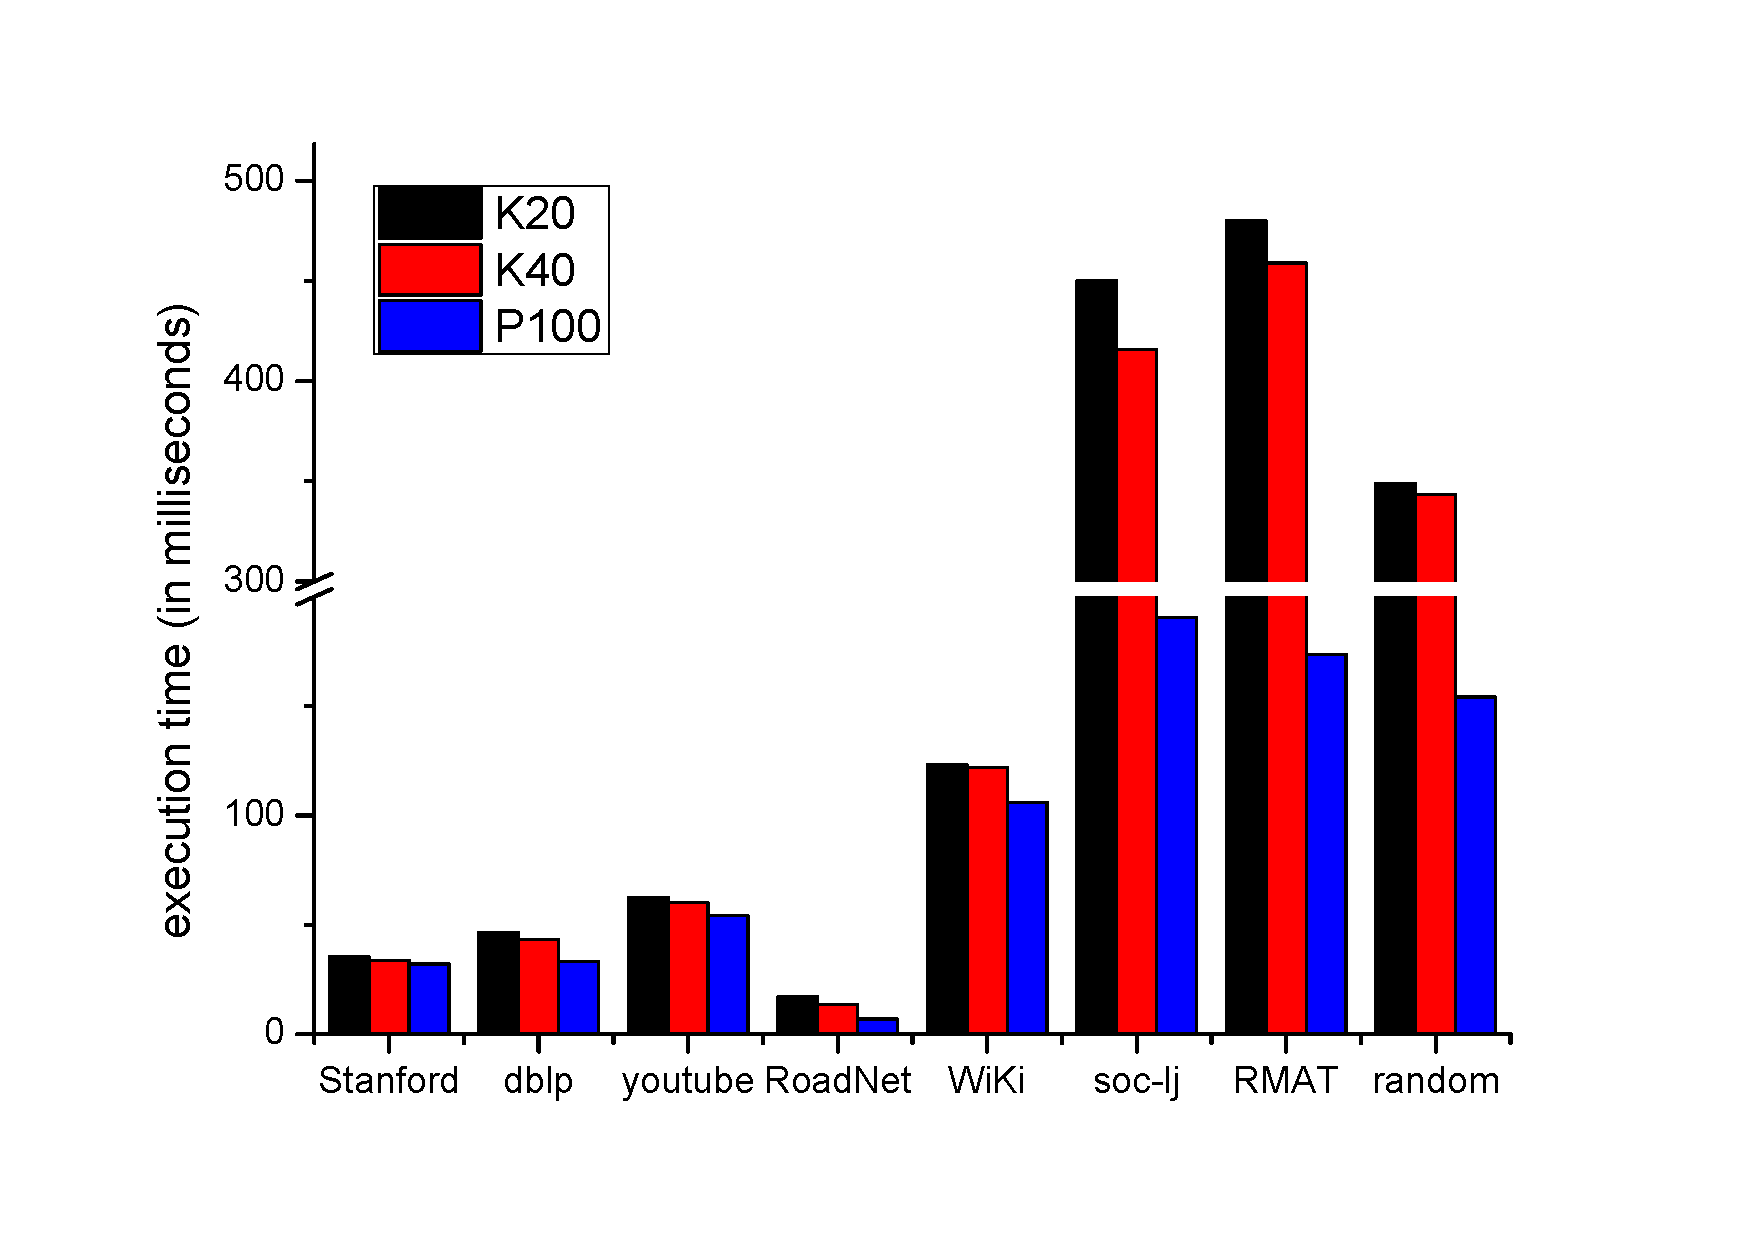
\includegraphics[scale=0.25]{figure/scale.pdf}
	\caption{The performance of Feluca on different GPU devices}
	\label{fig:scale}%
\end{figure}